\documentclass[internal]{nhitec_design}

\author{Antoine Mouchamps}
\date{\today}

\title{Tutoriel création de site web Laravel 
\includegraphics[height=20pt]{figures-logos/laravel.pdf}}

\frenchspacing % Parce que j'écris en français lol

\begin{document}

\VerbatimFootnotes{}
\maketitle
\newpage
{
\hypersetup{linkcolor=black}
\color{red_nhitec}
\tableofcontents
}

\newpage

\section{Introduction}

\subsection{Laravel, c'est quoi?}

\subsubsection{Prélude}

\laravel{}{} est ce qu'on appelle un \textit{framework}. C'est à dire un ensemble d'outil fournissant une architecture de base sur laquelle n'importe quel site web peut être bâti. A la fin de ce \textit{``petit''} tutoriel, vous serez je l'espère capable d'utiliser les fonctionnalités principales de Laravel, ainsi que les languages utilisés par ce framework et par la création de site web en général: \php{}, \html{} et en allant un petit peu plus loin, \css{}, \jquery{}  et \js{}. Cela parait beaucoup d'un coup, mais en y allant méthodiquement et pas à pas, ça devrait bien se passer!

Bon alors, et ce framework alors? Comment fonctionne-t'il?

\subsubsection{Fonctionnement \& philosophie}\label{sec:fonctionnement&philosophie}

\laravel{}{} utilise une architecture dite ``MVC'' (Modèle, Vue, Contrôleur) qui est décrite par la figure \textsc{Figure }\ref{fig:laravel_diagram}. Elle se base donc sur 4 concepts:
\begin{enumerate}
    \item \texttt{Routing:} Le routing est l'étape consistant à lier une URL, une \route{}, à une action spécifique, qui sera effectuée par une méthode (dans le sens \textit{Object-oriented-programming} du terme) contenue dans un \controller{}.
    \item \texttt{Controller:} Les \controllers{} sont donc appellés par les \texttt{routes}, ce sont eux qui vont s'occuper de manipuler les données, effectuer x-y-z tâches, et enfin d'envoyer une certaine \view{} à l'utilisateur.
    \item \texttt{View:} Le concept de \view{} est plutôt simple: Avec Laravel, chaque view correspond grosso-modo à une page que l'utilisateur voit affichée sur son écran.
    \item \texttt{Model:} Enfin, les données stockées dans la base de donnée ne sont pas traitées telles quelles. Laravel nous facilite la vie en associant chaque type de donnée à un \model{}, qui sera plus simple à utiliser par les \controllers{} et comportera des fonctionnalités très utiles.
\end{enumerate}

\begin{figure}[!h]
    \centering
    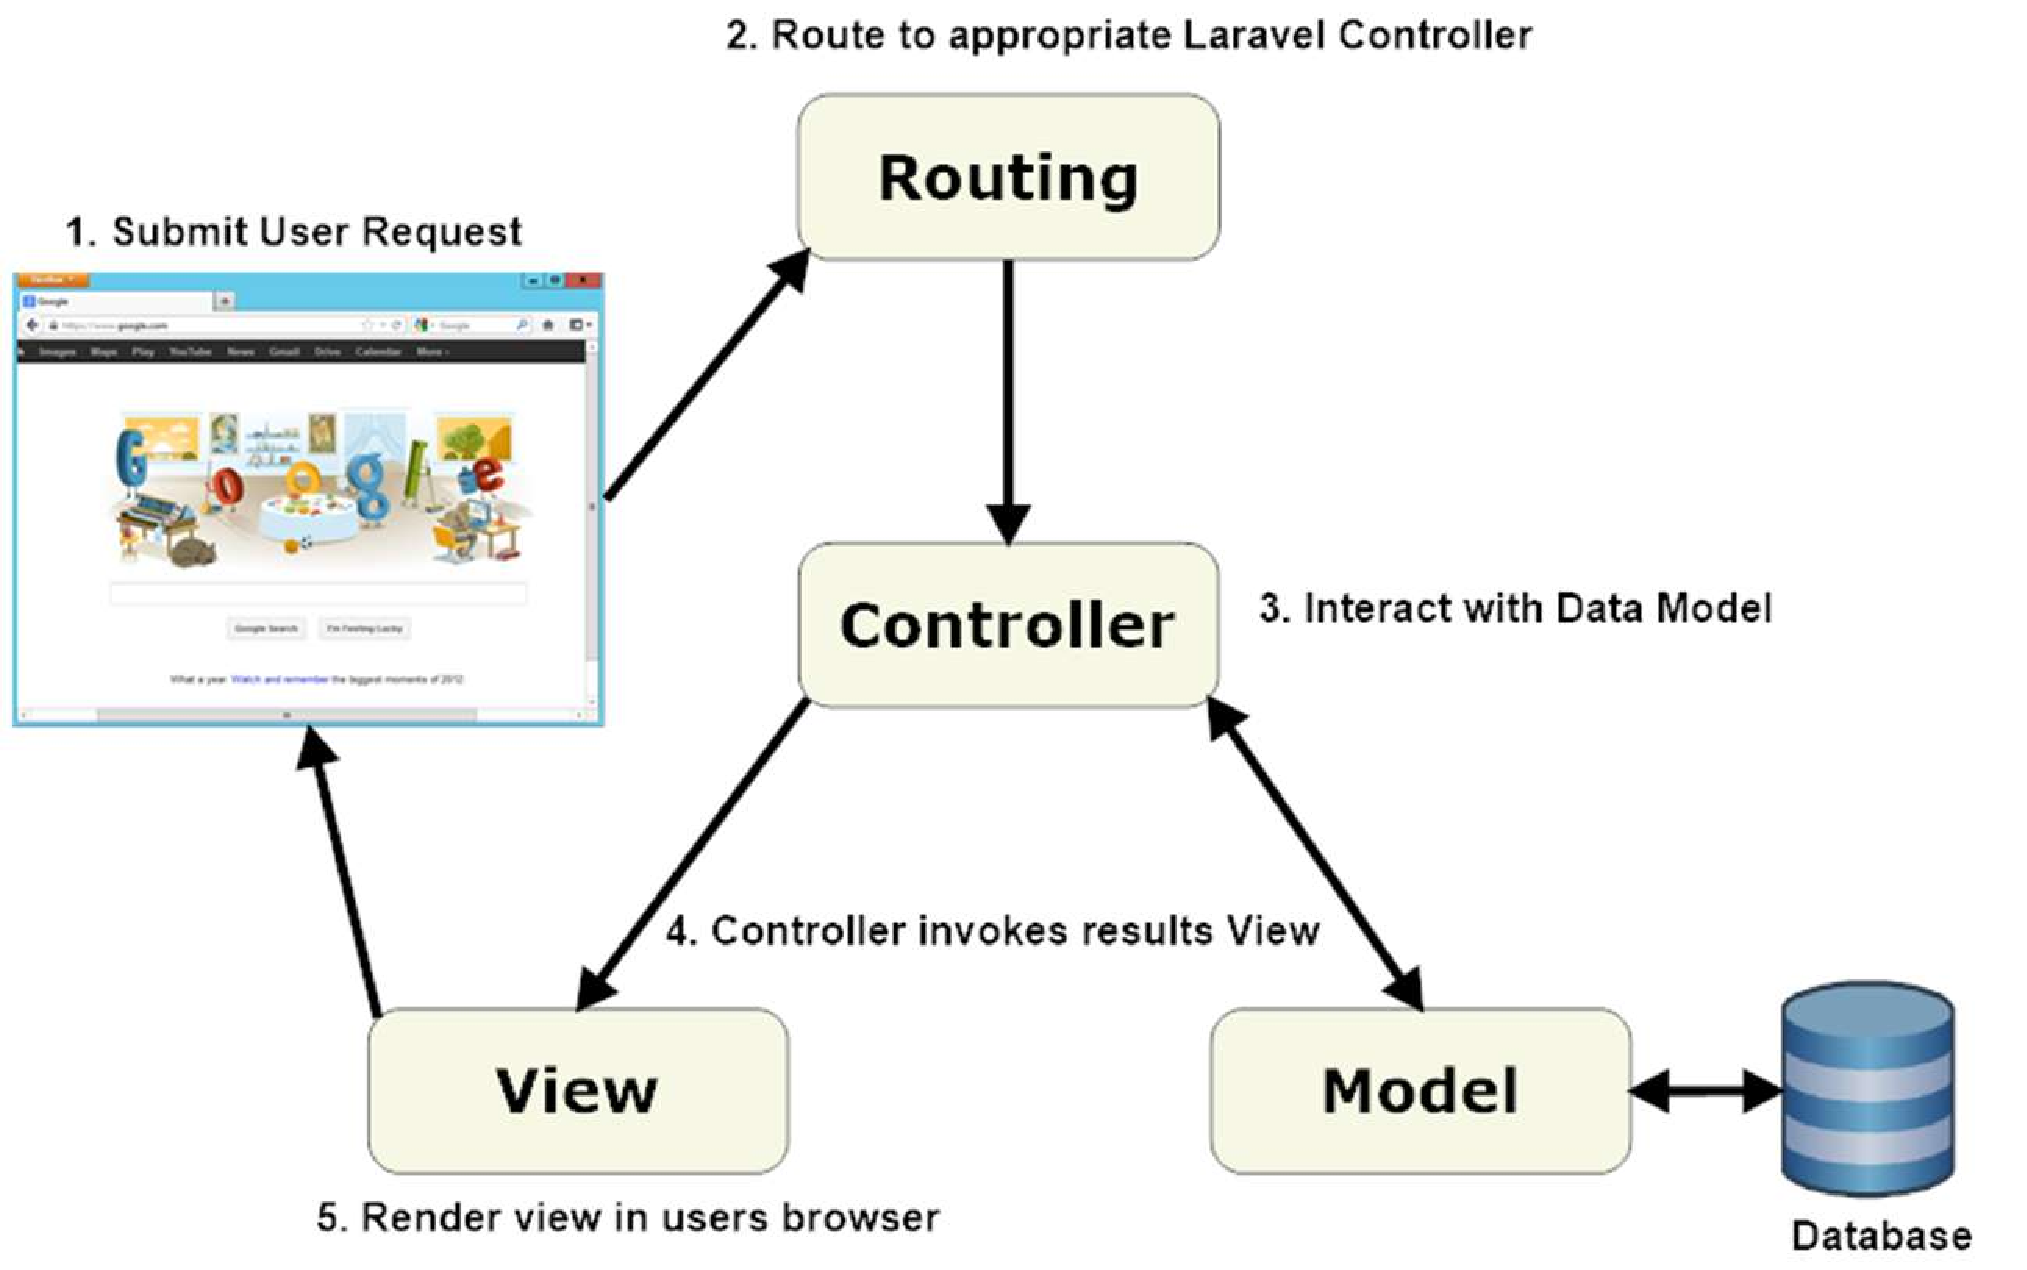
\includegraphics[width=0.5\textwidth]{figures-C1/diagram.pdf}
    \caption{\label{fig:laravel_diagram}}
\end{figure}

\newpage

\section{Premier site web}
\subsection{Setup initial}
Toute cette partie est normalement couverte par *insérer nom du doc pour la création d'un site laravel en utilisant Docker Desktop*. Normalement, à la suite de tutoriel, vous devriez avoir obtenu le site suivant en vous rendant sur \url{http://jsp}:
\begin{figure}[!h]
    \centering
    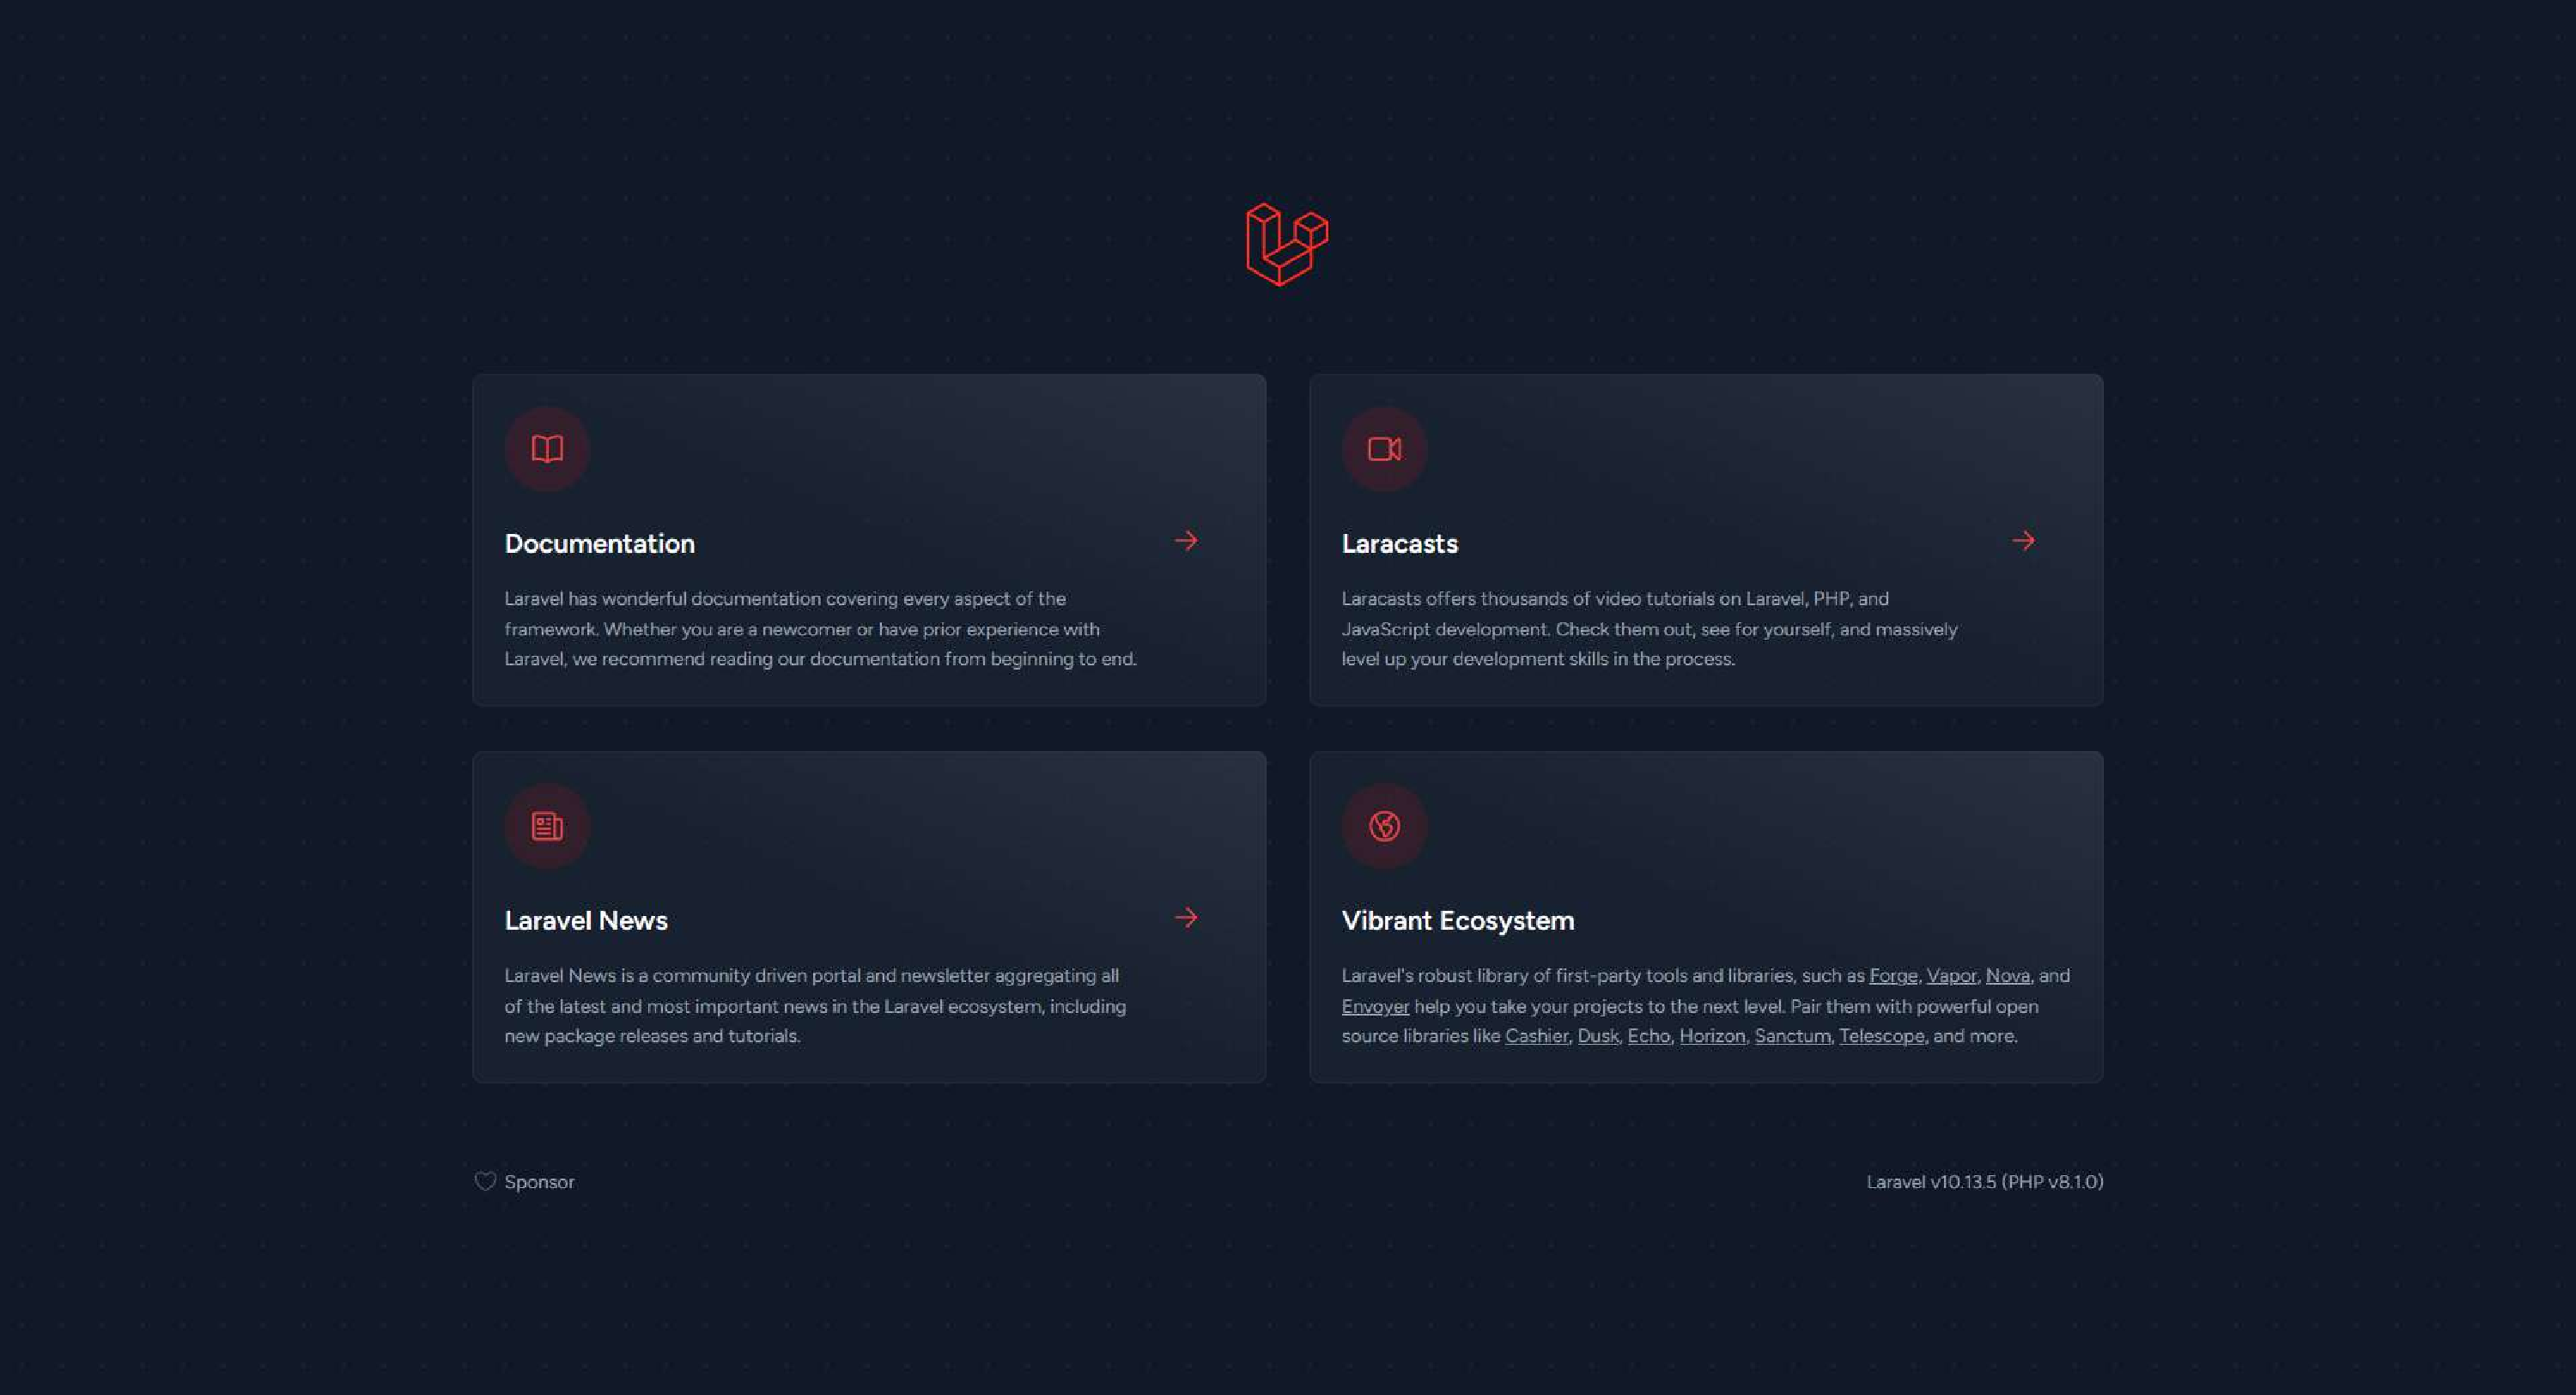
\includegraphics[width=0.75\textwidth]{figures-C1/laravel_default_website.pdf}
\end{figure}
Nous allons partir de ce site là. Pour ce tutoriel, mon projet sera appellé \texttt{tutorialstepbystep} donc son URL sera \url{http://tutorialstepbystep/}.

\subsection{Premières \routes{} \& \views{}}

\subsubsection{welcome!\label{sec:welcome!}}
Les \routes{} se trouvent dans le fichier \verb|routes\web.php|. \\
\begin{wrapfigure}[5]{r}{0.5\textwidth}
    \vspace{-0.5cm}
    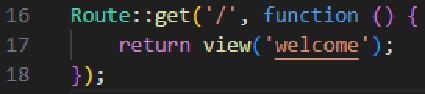
\includegraphics[width=0.5\textwidth]{figures-C1/basic_route.pdf}
\end{wrapfigure}
Dans ce fichier se trouve cette \route{} par défaut. Le premier argument de \verb|get()| est l'adresse (absolue) qui sera visée par la \route{}. En l'occurence, la fonction en deuxième argument sera exécutée lorsque l'URL est '/', donc \url{http://tutorialstepbystep/}. Remarquons que la fonction excécutée retourne la \view{} \textit{welcome}, c'est pourquoi nous voyons la page d'acceuil de laravel en nous rendant à cette adresse.

Allons voir le contenu de cette \view{}. Les \views{} en \laravel{} ne sont pas écrites en fichier \verb|.html| de base, mais sous la forme de fichiers \verb|fichier.blade.php|, qui permettent d'ajouter des fonctionnalités en plus\footnote{\textit{\underline{HINT:}} toutes les commandes commençant par un \verb|@| existent grâce au format \blade{}, ainsi que la commande \verb|{{}}|. Plus d'informations \href{https://laravel.com/docs/10.x/blade#blade-directives}{ici}.} à l'\html{} classique. 

Il y a bien beaucoup de chose dedans mais pas de panique: supprimons tout.

Plus précisément, ne gardons que ceci:

\begin{figure}[!h]
    \centering
    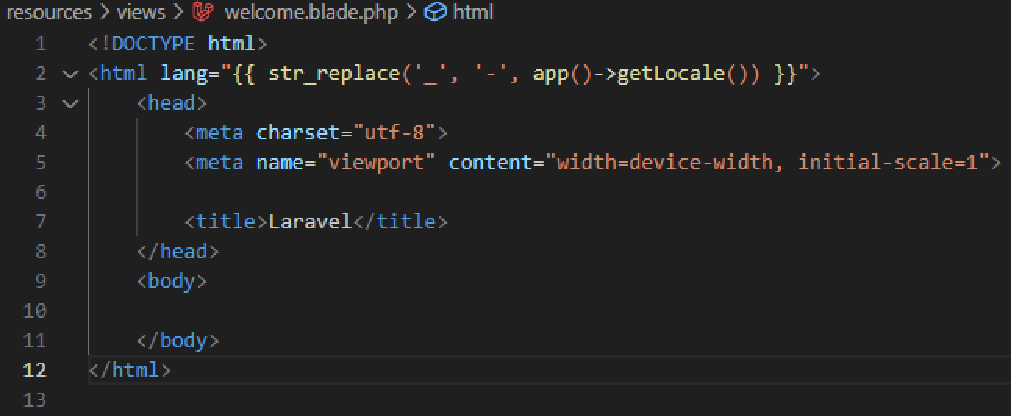
\includegraphics[width=\textwidth]{figures-C1/welcome_blade_empty.pdf}
\end{figure}

On y voit déjà plus clair. Dans ce qu'il reste, il n'y a que deux choses principales à retenir pour le moment: 
\begin{enumerate}
    \item le tag \verb|<head>| est l'endroit où les styles (\css{}) et scripts (\jquery{}  \& \js{}) sont importés, ainsi que 2-{}3 autres choses.
    \item le tag \verb|<body>| est le tag qui contiendra tout ce qui sera affiché par le navigateur. Donc pour le moment, en allant sur votre site, vous verrez une page vide.
\end{enumerate}

\subsubsection[Controller][laravel.com/docs/10.x/controllers\#introduction]{Controller}
Bon, il est temps de remplir tout ca. Commençons par créer un \controller{}. Pour cela, tapez
\verb|php artisan make:controller PagesController|\footnote{\verb|php artisan make:| est une commande très utile pour créer énormément de fichiers que nous verrons plus tard.}. Les \controllers{} se trouvent dans \verb|app\Http\controllers{}\|. Dans \verb|PagesController|, créez trois fonctions comme à la \textsc{Figure }\ref{fig:PagesController1}.

\begin{wrapfigure}[6]{r}{0.25\textwidth}
    \vspace{-0.5cm}
    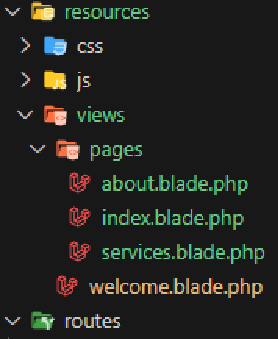
\includegraphics[width=0.25\textwidth]{figures-C1/3_premieres_views.pdf}
\end{wrapfigure}

Vous l'aurez compris, \verb|return view()| permet d'afficher la \view{} donnée en argument. En l'occurence, les 3 \views{} \verb|index|, \verb|services|, \verb|about| n'existent pas encore, il va donc falloir les créer! Notez également que \verb|pages.| indique que ces 3 \views{} se trouvent dans le dossier \verb|pages|. Par conséquent, vous pouvez commencer par créer les 3 fichiers dans un nouveau dossier comme à droite.

\newpage 
\SaveVerb{term}|PagesController|
\begin{wrapfigure}[16]{r}{0.5\textwidth}
    \centering
    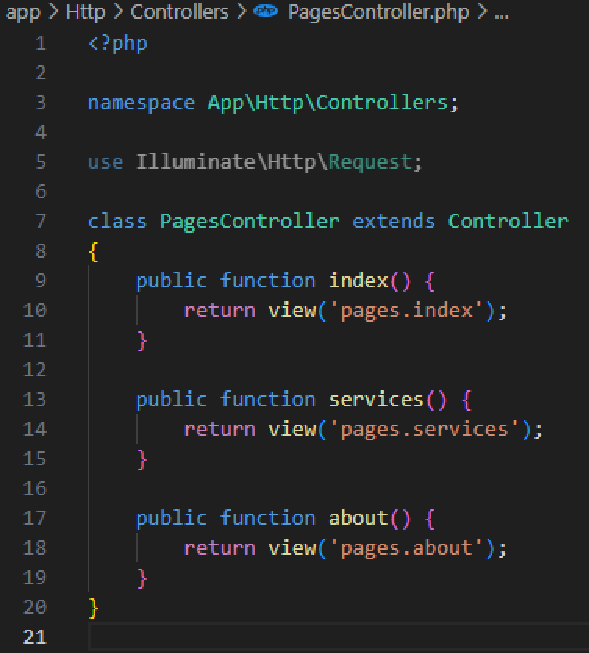
\includegraphics[width=0.5\textwidth]{figures-C1/pages_controller_1.pdf}
    \caption{\protect\UseVerb{term}\label{fig:PagesController1}}
\end{wrapfigure}
Si vous vous rappellez bien de ce qu'on a vu plus tôt, chaque \view{} \html{} doit contenir un tag \verb|<head>|. Celui-ci sera le même pour chaque page donc il serait judicieux\footnote{\textbf{D.R.Y}: \textit{Don't Repeat Yourself!}} de créer une sorte de template dans lequel on mettrait le \verb|<head>| et qui sera ensuite utilisé pour les 26854 pages que comptera bientôt notre site! 

COMME PAR HASARD les \views{} \verb|.blade.php| nous permettent de faire cela: commencez par créer un dossier \verb|layouts| dans les views, et créez un fichier dedans appellé \verb|app.blade.php|. Ensuite, remplissez-le avec le contenu de \verb|welcome.blade.php| (que vous pouvez désormais supprimer), puis ajoutez la commande \verb|@yield('content')| dans le \verb|<body>|. Enfin, il ne reste plus qu'a utiliser ce layout pour remplir vos 3 nouvelles \views{}.

\vspace{2cm}
\SaveVerb{about}|about|
\SaveVerb{services}|services|
\SaveVerb{index}|index|
\begin{figure}[!h]
    \centering
    \begin{subfigure}[b]{0.49\textwidth}
         \centering
         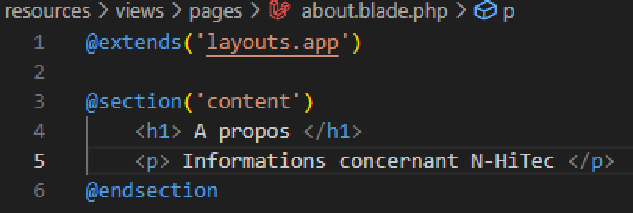
\includegraphics[width=\textwidth]{figures-C1/basic_about.pdf}
     \end{subfigure}
     \begin{subfigure}[b]{0.49\textwidth}
         \centering
         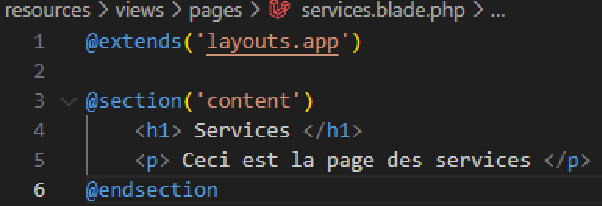
\includegraphics[width=\textwidth]{figures-C1/basic_services.pdf}
     \end{subfigure}
     \begin{subfigure}[b]{1\textwidth}
         \centering
         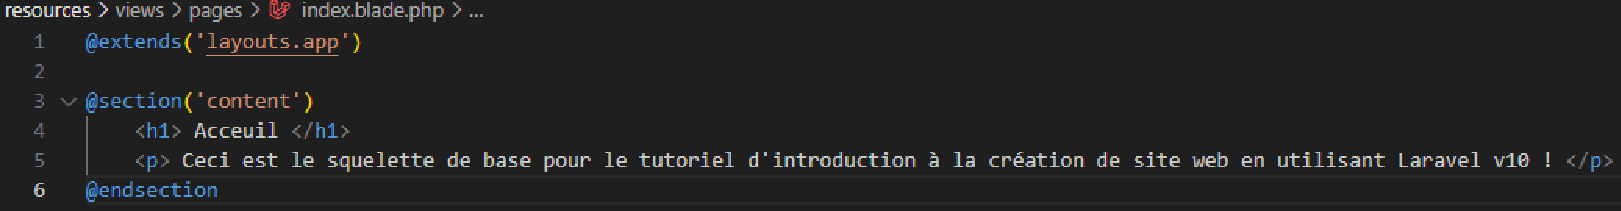
\includegraphics[width=\textwidth]{figures-C1/basic_acceuil.pdf}
     \end{subfigure}
        \caption{Contenu des \views{} \protect\UseVerb{about} (à gauche), \protect\UseVerb{services} (à droite) et \protect\UseVerb{index} (en bas)}
\end{figure}
Petit tuto \html{} rapide: le tag \verb|<p>| renferme un pparagraphe, et le tag \verb|<h1>| contient lui un h1titre. De même, \verb|<h2>| désignera un h2sous-titre, \verb|<h3>| un h3sous-sous-titre, \verb|<h4>| un h4sous-sous-sous-titre, \ldots

Que se passe-t'il exactement? Chacune des \views{} va prendre le contenu du layout \verb|app| (via \verb|@extends()|), et remplir sa section \verb|content| par ce qu'il y a entre \verb|@section| et \verb|@endsection|. Simple et efficace! Nous rajouterons d'autres choses dans ce layout par la suite.

\newpage

Enfin, pour pouvoir admirer le fruit de votre dur labeur, il faut créer les \routes{} qui permettront d'afficher ces pages. Pour cela, rendez-vous dans \verb|web.php|:

\begin{wrapfigure}[15]{r}{0.7\textwidth}
    \vspace{-0.5cm}
    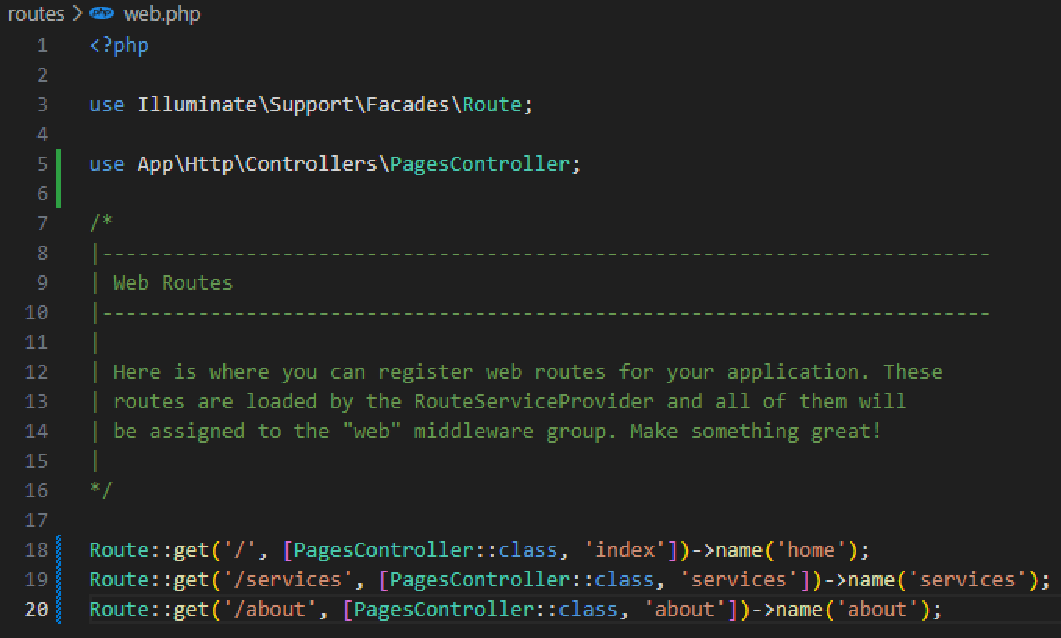
\includegraphics[width=0.7\textwidth]{figures-C1/3_premieres_routes.pdf}
\end{wrapfigure}
Afin d'utiliser notre nouveau controller, il faut le déclarer pour que \laravel{} sache qu'il existe. C'est à ca que sert ``\verb|use gngngn|'', (ce qui est suit est plutôt évident).
Ensuite, décortiquons ce qui se passe: Comme précédement, le 1er argument de \verb|get()| donne l'adresse. Par exemple, la 2eme route est appellée à l'URL \url{http://tutorialstepbystep/services}. Le deuxième argument donne dans un tableau le \controller{} ainsi que sa méthode à exécuter. Pour la deuxième route, aller à l'URL mensionnée va donc exécuter la fonction \verb|services()| que nous avons créée il y a 5 (ou 40) minutes. Celle ci nous retourne la \view{} correspondante, donc en allant sur cet URL nous voyons dans un coin de l'écran:

\begin{figure}[!h]
    \centering
    \fbox{
\includegraphics[]{figures-C1/basic_services_web.pdf}}
    \caption{page internet moche}
\end{figure}

C'est laid, pas vrai? Nous allons améliorer cela à la prochaine section.

\newpage

\subsection[Bootstrap et CSS]{\bs{} \& \css{}}
\subsubsection[Qu'est-ce que le CSS?][fr.wikipedia.org/wiki/Feuilles\_de\_style\_en\_cascade]{Qu'est-ce que le \css{}?}\label{sec:css} 
\textit{``De la même façon que HTML, CSS\footnote{Cascading Style Sheets} n'est pas vraiment un langage de programmation. C'est un langage de feuille de style, c'est-à-dire qu'il permet d'appliquer des styles sur différents éléments sélectionnés dans un document HTML''.} (\href{https://developer.mozilla.org/fr/docs/Learn/Getting_started_with_the_web/CSS_basics}{developer.mozilla.org}). Cela signifie que le \css{} est le langage utilisé pour décrire comment chaque élément \html{} doit être affiché. Cela va de la taille et couleur du texte à la création de \verb|navbar|, \verb|buttons|, \verb|tables|, etc\ldots en passant par diverses animations simples ou plus complexes.

Le langage suit la philosophie suivante: à chaque sélecteur, on associe des propriétés. Les sélecteurs peuvent être des tags \html{} eux-mêmes, des \verb|class|, \verb|id|, ou d'autres choses. Ua bonne pratique est de styliser un maximum de composants en créant une multitude de \verb|class| ayant chacune une tâche spécifique (taille, couleur, etc) afin d'obtenir une structure générale et modulaire, et ensuite d'assigner autant de \verb|class| que l'on veut aux tags \html{} que l'on souhaite modifier. Plus de détails dans la section dédiées (WIP).

\subsubsection[A quoi sert Bootstrap?][fr.wikipedia.org/wiki/Bootstrap\_(framework)]{A quoi sert \bs{}?}
Autant dire que la philosophie décrite conduit très rapidement à des fichiers énormes (milliers de lignes), illisibles, de successions de sélecteurs-propriétés, ce qui conduit à une maintenance plus que laborieuse, alors que là n'est souvent pas la partie sur laquelle les développeurs veulent passer du temps (sauf si c'est leur métier, évidement\footnote{on parle alros de développeurs \textit{front-end}.}). C'est pour cela que de nombreux \textit{frameworks front-end} existent afin d'amener de nombreuses \verb|class| et plugins \js{} prédéfinis. En l'occurence, nous allons utiliser \bs{}, qui est un \textit{framework} utilisé pour construire des sites de manière \textit{responsive\footnote{\textit{responsive} signifie que le site/composant adapte son rendu en fonction de la taille de l'écran, du format etc, ce qui est quand même très important.}} rapidement et facilement.

Pour plus de renseignement et pour découvrir les fonctionnalités de \bs{}, rendez-vous sur \href{https://getbootstrap.com/docs/5.3/getting-started/introduction/}{Doc \bs{}}. Dans la \texttt{Section } et dans votre futur, vous utiliserez énormément de \verb|class| \bs. Il est donc imporant de se familiariser avec rapidement, par exemple en lisant la documentation des \verb|class| que vous ne connaissez pas, même si c'est fort déroutant au début afin que cela roule tout seul à moyen terme.

\subsubsection[Vite? Comme la rapidité de cette formation?][laravel.com/docs/10.x/vite\#introduction]{\vite{}? Comme la rapidité de cette formation?}
Les \textit{frameworks} ``règlent le problème'' des 10000 lignes de code à écrire, mais pas celui de leur gestion et compilation. Rentre alors en scène \vite:

\textit{``Vite is a modern frontend build tool that provides an extremely fast development environment and bundles your code for production\footnote{\textit{production} signifie le déploiement du site pour le public}. When building applications with Laravel, you will typically use Vite to bundle your application's CSS and JavaScript files into production ready assets''.} (\href{https://laravel.com/docs/10.x/vite#introduction}{Doc \laravel{}})
\subsubsection{Installation}

Pour installer \bs{}, il suffit d'exécuter les commandes suivantes:
\begin{enumerate}
    \item \verb|npm install bootstrap @popperjs/core|, qui permet d'installer \verb|Popper|, une bibliothèque \js{} utilisé par \bs{}.
    \item \verb|npm install sass --save-dev|, qui permet d'utiliser le langage \sass{}, utilisé par \\ \bs{}.
\end{enumerate}

\begin{wrapfigure}[18]{r}{0.35\textwidth}
    \vspace{-0.5cm}
    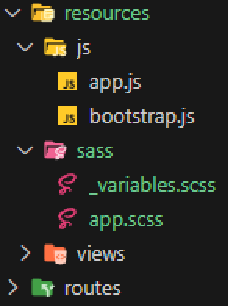
\includegraphics[width=0.35\textwidth]{figures-C1/bs_setup.pdf}
    \caption{\label{fig:bs_setup}}
\end{wrapfigure}
Ensuite, dans le dossier \verb|resources|, nous allons renommer le dossier \verb|css| en \verb|sass| et le fichier \verb|app.css| à l'intérieur en un fichier \verb|app.scss|. Il nous reste ensuite à ajouter un fichier \verb|_variables.scss| dans le dossier \verb|sass|, que nous utiliserons plus tard. Pour l'instant, nous allons juste le remplir avec le contenu de la \texttt{Figure~\ref{fig:variables.scss}}. Vous devriez donc obtenir un arrangement comme à la \textsc{Figure~\ref{fig:bs_setup}}. Comme nous l'avons vu VOIRSECTION, le fichier \verb|app.scss| est compilé par \vite{} en un fichier \css{} dans le dossier \verb|public| qui permettra de custommiser notre site web. Il faut donc le remplir par ce qui est donné par la \textsc{Figure }\ref{fig:app.scss}, où la première ligne permet de changer la police d'écriture utilisée par défaut (avec celle ajoutée dans \verb|_variables.scss|), la deuxième importe le fichier \verb|variables.scss| que nous venons de créer (qui pour le moment est vide) et enfin la troisième importe toutes les fonctionnalités de \bs{}. Nous verrons dans une future section (WIP) comment personnaliser ces importations pour n'importer que les fonctionnalités que l'on utilise, et donc gagner en performances. 

Par ailleurs, lorsque nous créerons des codes \sass{} custom, nous les utiliserons en les importants dans ce fichier.

\begin{figure}[!h]
    \begin{minipage}{0.44\textwidth}
        \centering
        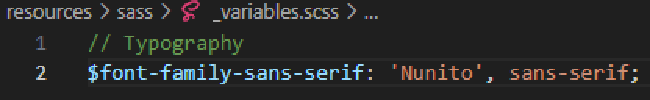
\includegraphics[width=\textwidth]{figures-C1/variables.pdf}
        \caption{\label{fig:variables.scss}}
    \end{minipage} 
    \begin{minipage}{0.54\textwidth}
        \centering
        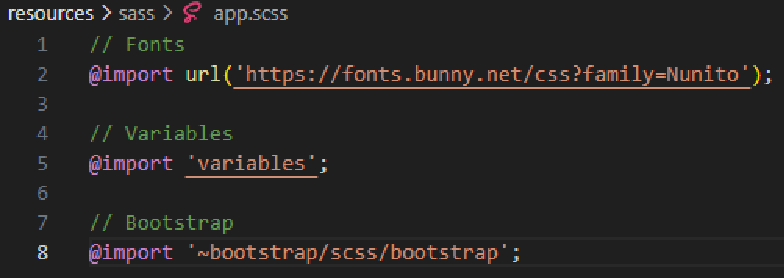
\includegraphics[width=\textwidth]{figures-C1/app.scss.pdf}
        \caption{\label{fig:app.scss}}
    \end{minipage}
\end{figure}

En ce qui concerne le code \js{} utilisé par \bs{}, il faut l'importer en ajoutant \verb|import * as bootstrap from 'bootstrap'| dans le fichier \verb|resources/js/app.js|.
\newpage

\begin{wrapfigure}[8]{r}{0.65\textwidth}
    \vspace{-0.5cm}
    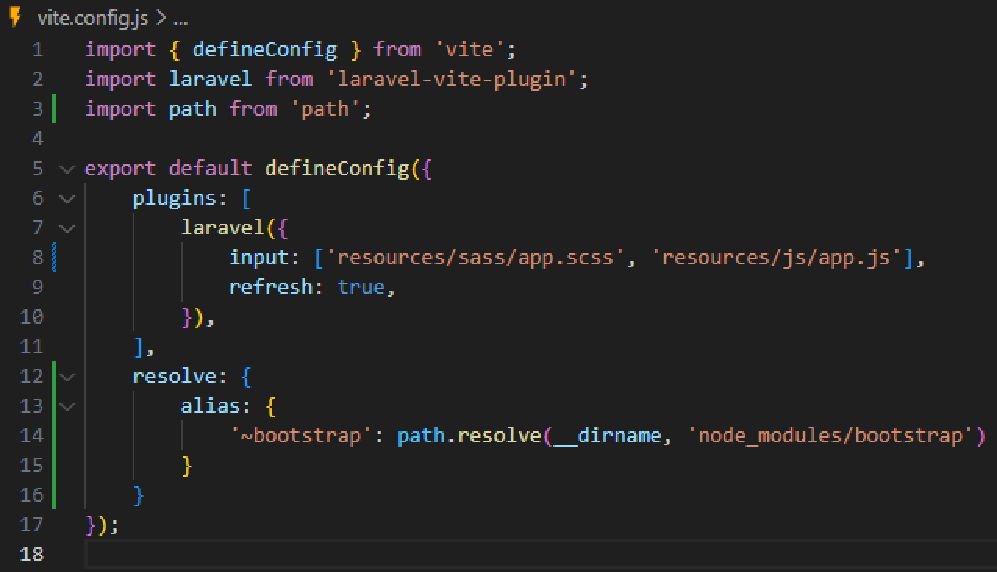
\includegraphics[width=0.65\textwidth]{figures-C1/vite.config.pdf}
\end{wrapfigure}

Enfin, il faut modifier les paramètres de \vite{} pour prendre en compte les changements que nous avons mis en place. Modifier donc la ligne 8 et ajoutez d'autres lignes dans le fichier \verb|vite.config.js| situé dans le dossier racine du site.

\vspace{3cm}

\begin{wrapfigure}[11]{r}{0.65\textwidth}
    \vspace{-0.5cm}
    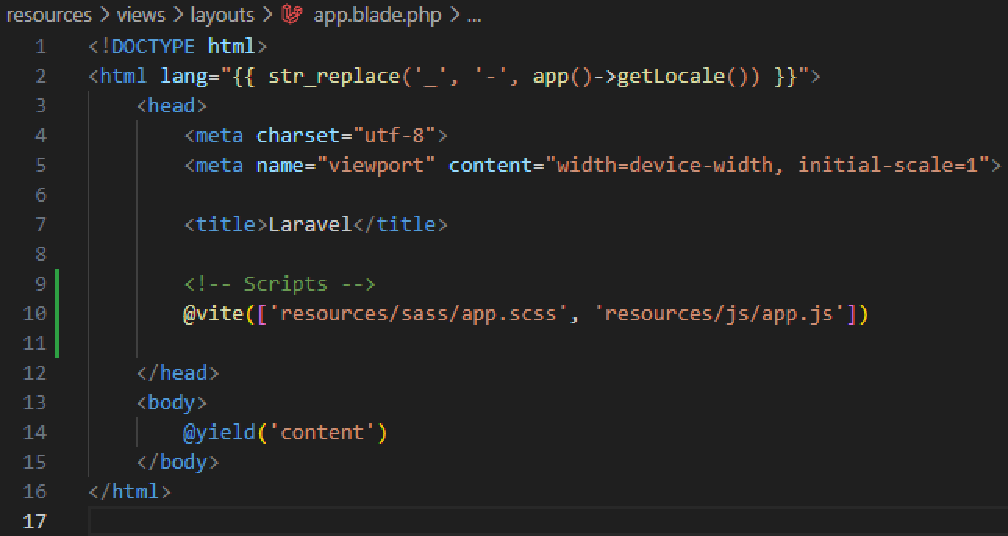
\includegraphics[width=0.65\textwidth]{figures-C1/vite_in_layout.pdf}
\end{wrapfigure}

Remarquez que jusqu'ici, on ne voit toujours pas de changement quant on va sur notre site. La raison est que nous n'avons pas encore ``dit'' à nos \views{} d'utiliser nos ajouts (jusqu'ici, seulement le changement de police). Pour cela, rendez-vous dans notre layout (càd \verb|app.blade.php|) et ajoutons la ligne suivante:

\vspace{1.1cm}
Maintenant, tout est prêt pour commencer à utiliser \bs{}.

\subsubsection{Utilisation}

Comme expliqué plus haut, \bs{} nous fournit une multitude de \verb|class| que nous pouvons utiliser pour styliser nos \textit{tags} \html{}. Modifions donc nos \blades{} \verb|about.blade.php| et \verb|index.blade.php| comme ceci:

\SaveVerb{about}|about.blade.php|
\SaveVerb{index}|index.blade.php|
\begin{figure}[!ht]
    \centering
    \begin{minipage}{0.28\textwidth}
         \centering
         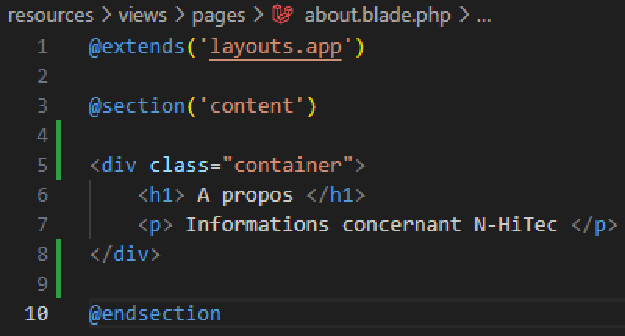
\includegraphics[width=\textwidth]{figures-C1/about_bs.pdf}
         \caption{\\\hspace{\textwidth} \protect\UseVerb{about}}
    \end{minipage}
    \begin{minipage}{0.7\textwidth}
         \centering
         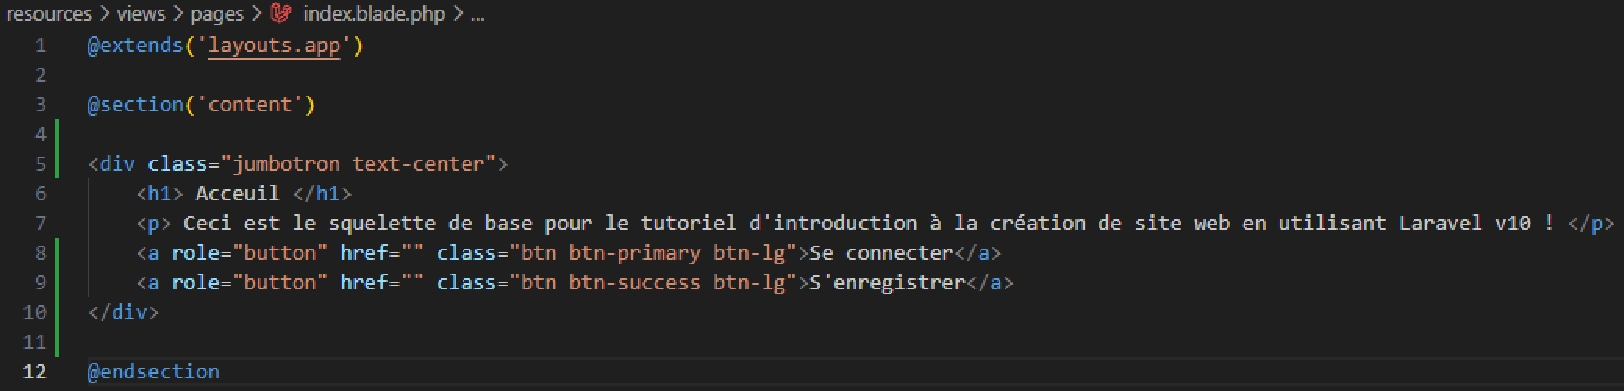
\includegraphics[width=\textwidth]{figures-C1/index_bs.pdf}
         \caption{\protect\UseVerb{index}\label{fig:index_bs}}
    \end{minipage}
\end{figure}

Par exemple, dans la \texttt{Figure~\ref{fig:index_bs}}, \verb|class="text-center"| assigne la classe \verb|text-center| à l'élément, et en maintenant la touche \textit{Ctl} enfoncée et en passant le curseur sur la classe, vous verrez ceci:

\begin{wrapfigure}[3]{r}{0.55\textwidth}
    \vspace{-0.5cm}
    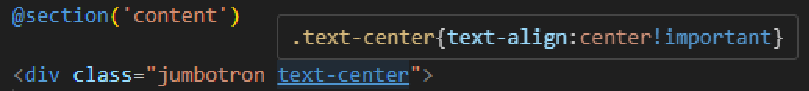
\includegraphics[width=0.55\textwidth]{figures-C1/see_class.pdf}
\end{wrapfigure}
Dans le petit cadre, nous voyons le code \css{}\footnote{voir \texttt{Section~\ref{sec:css}}} correspondant à cette classe. Concrètement, cette \verb|class| permet de centrer l'élément dans son conteneur.

Pour la customisation de la page des services, nous allons en profiter pour découvrir une nouvelle mécanique: passer des données aux pages. En effet, c'est quand même pratique de pouvoir afficher des informations dynamiquement! Pour le moment, nous n'allons pas encore s'embêter avec la base de donnée, nous allons juste voir comment la mécanique de base fonctionne. Rappelez-vous de la \texttt{Section~\ref{sec:fonctionnement&philosophie}}, ce sont les \controllers{} qui s'occupent de manipuler les données avant d'afficher une \view{}. Dès lors, c'est dans la fonction \verb|services()| de \verb|PagesController.php| que nous allons ajouter des choses:
\begin{figure}[!h]
    \centering
    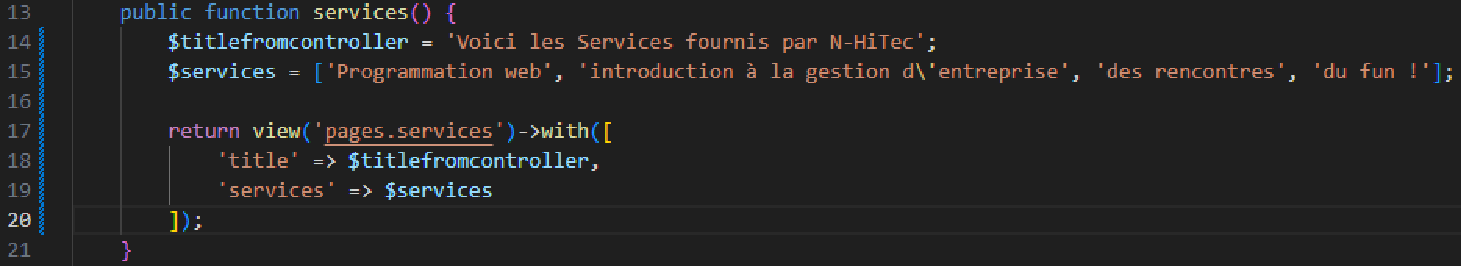
\includegraphics[width=\textwidth]{figures-C1/services_fct_bs.pdf}
\end{figure}

\verb|$titlefromcontroller| et \verb|$services| sont 2 variables, et nous les passons à la \view{} par l'intermédiaire du \verb|->with(...)|. 

\begin{wrapfigure}[6]{r}{0.5\textwidth}
\vspace{-0.5cm}
    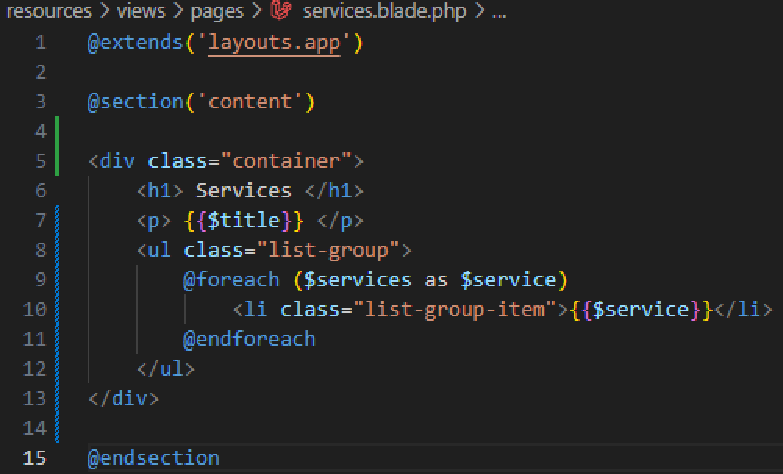
\includegraphics[width=0.5\textwidth]{figures-C1/services_bs.pdf}
\end{wrapfigure}

Ensuite, nous pouvons utiliser les variables \verb|title| et \verb|services| dans la\blade{} concernée. Dans la \texttt{Section~\ref{sec:welcome!}} nous avons pris connaissance des avantages du format \verb|.blade.php|. Celui-ci nous apporte donc les commandes \verb|{{}}|\footnote{Cette commande agit comme un \verb|printf()| en C. Elle permet d'afficher le contenu de la variable en argument.} et \verb|@foreach()|\footnote{Boucle \verb|foreach| classique, pour itérer sur un tableau. Les tags \verb|<a>| ainsi que \verb|<ul>| et \verb|<li>| seront expliqué à la section suivante.}.

\newpage

Et voilà! Maintenant, il suffit de taper \verb|npm run dev|\footnote{Cette commande permet de compiler le \css{} et \js{} en créant un mini serveur localement. Cette commande utilisée lors du \underline{DEVELOPPEMENT DU SITE} permet d'appliquer les modifications apportées à des fichiers rapidement sans devoir refresh la page. Plus d'infos sur les commandes de \vite{} à la \texttt{Section~} (WIP).} pour admirer le résultat. C'est déjà vachement mieux, non?

\begin{figure}[!h]
    \begin{subfigure}[c]{0.73\textwidth}
        \fbox{
\includegraphics[width=\textwidth]{figures-C1/web_index.pdf}}
    \end{subfigure}\hfill
    \begin{subfigure}[c]{0.24\textwidth}
        \caption{\url{http://tutorialstepbystep/}} 
    \end{subfigure}
    \begin{subfigure}[c]{0.73\textwidth}
        \fbox{
\includegraphics[width=\textwidth]{figures-C1/web_about.pdf}}
    \end{subfigure}\hfill
    \begin{subfigure}[c]{0.24\textwidth}
        \caption{\url{http://tutorialstepbystep/about}} 
    \end{subfigure}
    \begin{subfigure}[c]{0.73\textwidth}
        \fbox{
\includegraphics[width=\textwidth]{figures-C1/web_services.pdf}}
    \end{subfigure}\hfill
    \begin{subfigure}[c]{0.24\textwidth}
        \caption{\url{http://tutorialstepbystep/services}} 
    \end{subfigure}
    \caption{3 pages créées jusqu'à présent et stylisées avec \bs{}.}
\end{figure}
C'est bien beau, mais jusque ici le seul moyen de naviguer entre les pages est de rentrer leur URL, ce qui n'est ma foi pas fort pratique. Remédions à cela avant de passer à la suite.

\subsubsection{Navbar}

C'est un gros morceau qui utilise beaucoup des \verb|class| de \bs{}, donc il va falloir s'accrocher. D'abord, créez un dossier \verb|inc| dans \verb|resources/views| et un fichier \verb|navbar.blade.php| dans ce nouveau dossier. Remplissez ce fichier comme la \texttt{Figure~\ref{fig:navbar}}.

\begin{figure}[!h]
    \centering
    \begin{minipage}{0.7\textwidth}
         \centering
         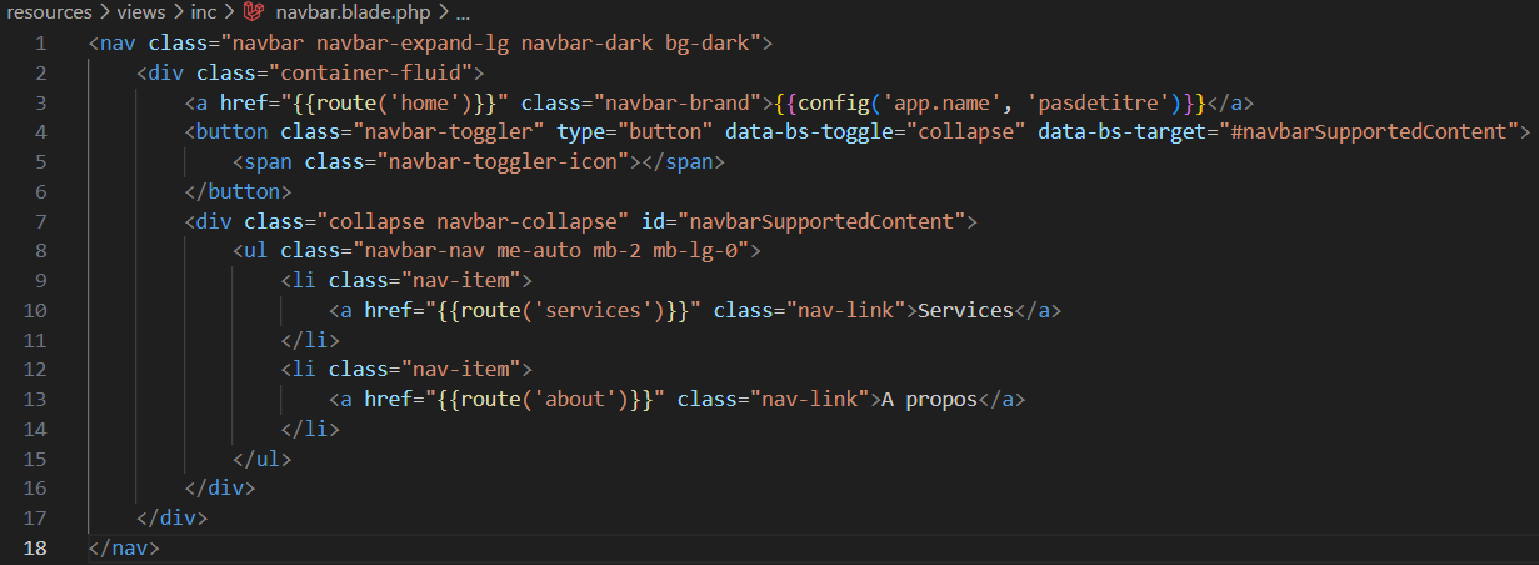
\includegraphics[width=\textwidth]{figures-C1/navbar.pdf}
         \caption{\label{fig:navbar}}
    \end{minipage}
    \begin{minipage}{0.28\textwidth}
         \centering
         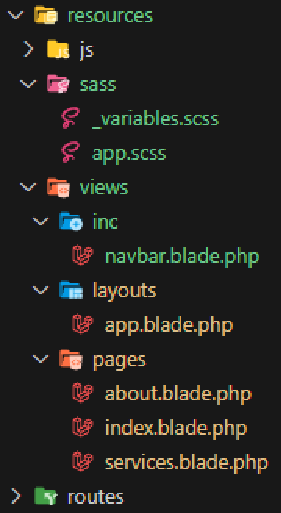
\includegraphics[width=0.5\textwidth]{figures-C1/navbar_file.pdf}
         \caption{}
    \end{minipage}
\end{figure}

\begin{wrapfigure}[2]{r}{0.3\textwidth}
    \vspace{-0.5cm}
    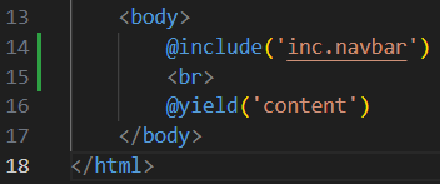
\includegraphics[width=0.3\textwidth]{figures-C1/navbar_layout.pdf}
\end{wrapfigure}

Ensuite, il faut ajouter notre \textit{navbar} à notre \textit{layout} afin qu'elle apparaisse sur toutes nos pages. Pour cela, rien de plus simple! 
\vspace{2cm}

\newpage

Qu'est ce que c'est que tout ça? Décomposons tout cela.
Premièrement, nous découvrons ici trois nouveaux tags \html{}:
\begin{enumerate}
    \item \verb|<a>| est un tag permettant la création d'un lien vers une autre URL, que l'on place dans l'attribut \verb|href|. Au lieu de tapez l'URL d'une \route{}, \laravel{} nous permet d'optimiser l'écriture en utilisant la commande \verb|route('nomdelaroute')| afin d'obtenir l'URL en question.~\verb|{{...}}| permet ensuite de l' ``afficher'' dans le \verb|href|.
    \item \verb|<ul>| est un tag signifiant la création d'une liste.
    \item \verb|<li>| représente un élément d'une liste.
\end{enumerate}

Pour le reste je vous invite à lire ce que font chaque \verb|class| et de jeter un oeil sur \href{https://getbootstrap.com/docs/5.3/components/navbar/}{la doc \bs{} sur les navbars}. Bien que ça soit indigeste lors d'une première lecture, ça l'est beaucoup moins que si nous devions analyser les \verb|class| une par une\ldots

Néanmoins, quelques notions clées: 
\begin{itemize}
    \item \textit{``collapsing''} fait référence au fait de faire disparaitre la navbar au profit d'une liste déroulable avec un bouton lorsque la largeur de l'écran devient plus petit qu'une valeure fixée (ici, $992\mathrm{px}$ car on utilise le mot clé \verb|lg|).
    \item le boutton spécial pour dérouler la navbar est créé par le tag \verb|<button class="navbar-toggler>|, qui est invisible lorsque la largeur de l'écran est > $992\mathrm{px}$.
    \item rien à voir avec \bs{}, \verb|config()| permet d'accéder à certaines valeurs, notament celles du \verb|.env|. En l'occurence, \verb|'app.name'| permet d'accéder à \verb|APP_NAME| (et si cette valeur n'existe pas, le deuxième argument est affiché).
\end{itemize}

Dans la \texttt{Section} (WIP), nous verrons comment améliorer cette navbar. En attendant, voilà ce à quoi elle devrait ressembler:

\begin{figure}[!h]
    \centering
    \begin{minipage}[b]{0.9\textwidth}
        \centering
        \fbox{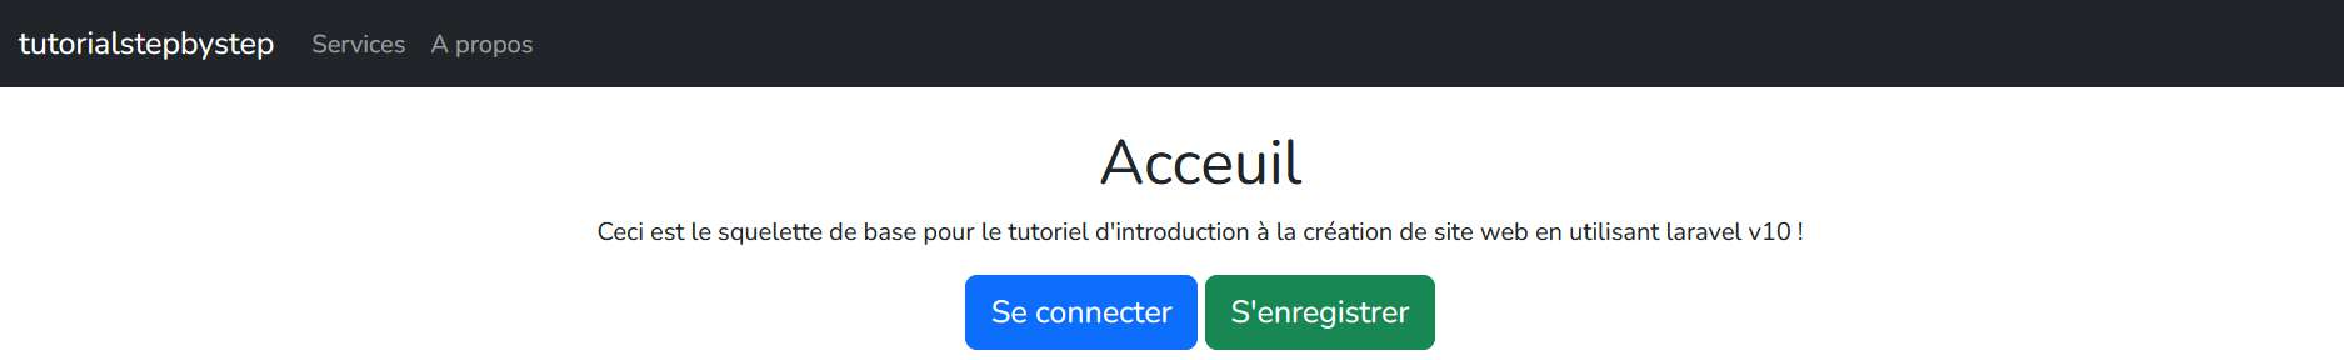
\includegraphics[width=\textwidth]{figures-C1/navbar_full.pdf}}
        \caption{navbar sur un écran de largeur $>992\mathrm{px}$}
    \end{minipage}
    \begin{minipage}[b]{0.44\textwidth}
        \centering
        \fbox{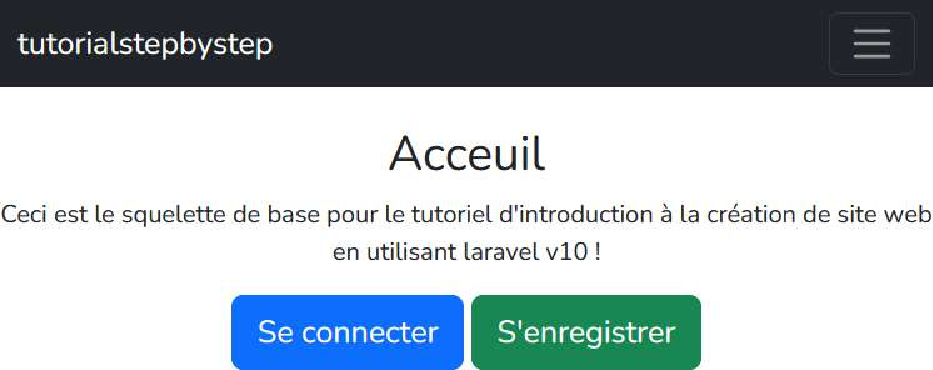
\includegraphics[width=\textwidth]{figures-C1/navbar_full_phone_2.pdf}}
        \captionsetup{justification=centering}
        \captionof{figure}{navbar vue depuis un téléphone (largeur $<992\mathrm{px}$)}
    \end{minipage}
    \hspace{0.1cm}
    \begin{minipage}[b]{0.44\textwidth}
        \centering
        \fbox{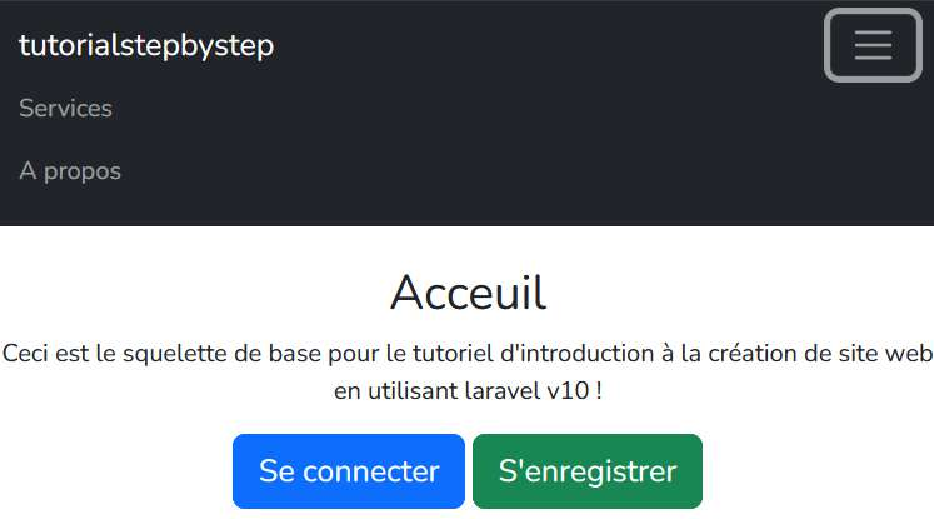
\includegraphics[width=\textwidth]{figures-C1/navbar_full_phone_1.pdf}}
        \captionsetup{justification=centering}
        \captionof{figure}{navbar en ayant appuyé sur le bouton en haut à droite}
    \end{minipage}
\end{figure}

\newpage

\subsection{Base de donnée}
Nous allons créer une base de donnée en utilisant l'exemple de posts sur un blog.


\subsubsection[PHPMyAdmin][]{\phpmyadmin{}}
\phpmyadmin{} est un site/logiciel permettant à des ignares comme nou\ldots comme vous* de manipuler des bases de données facilement sans connaissances en \mysql. Pour l'instant, nous allons configurer le \verb|.env| de notre site pour acceuillir une base de donnée et ensuite créer celle-ci grâce à \phpmyadmin{} (normalement ca ca sera fait ds le tuto d'installation en fait\ldots).

\subsubsection[Models][laravel.com/docs/10.x/eloquent\#generating-model-classes]{Models}
Comme dit dans la \texttt{Section~\ref{sec:fonctionnement&philosophie}}, le \model{} est l'objet qui nous permettra d'intéragir avec les \textit{posts} stockés dans notre base de donnée\footnote{pour chaque nouvel objet, on aura un \model{} correspondant}. Pour le créer, tapez \verb|php artisan make:model Post -m|, et observez la création d'un fichier \verb|Post.php| dans \verb|app/Models/|. Pour le moment, la class (au sens \php{} du terme) est vide, mais on peut ajouter des methods spécifique à ce \model{}, ce qui, nous le verrons (WIP), est très pratique.

\subsubsection[Migrations][laravel.com/docs/10.x/migrations\#introduction]{Migrations: comme les oiseaux?}

Une \migration{} est un fichier qui permet de définir les \tables{} de notre base de donnée. Une \table{} est grosso modo un type de donnée que la \db{} va stocker. Par exemple, la liste de tous les utilisateurs est une \table{}, tout comme les \textit{posts} que nous allons créer. Chaque \table{} contient un certain nombre de \columns{} qui elles sont les données stockées en temps que telles. En l'occurence, notre \table{} de \textit{posts} doit contenir une \column{} pour le titre d'un \textit{post} et une pour son contenu en lui même\footnote{Tous ces termes sont compliqués à décrire avec des mots, mais sont en réalité très intuitifs quand on imagine les données affichées dans un grand tableau à double entrée.}.

Pour créer notre migration, tapez \verb|rien du tout| car en fait, la \migration{} a été créée en même temps que notre \model{}! Elle se trouve dans \\\verb|database/migration/xxxx_xx_xx_xxxxxx_create_posts_table.php|. \\Ensuite, remplissez là comme à la \texttt{Figure~\ref{fig:basic_migration}}\footnote{lignes 16 et 17, de rien}:

Analysons tout a:
\begin{itemize}
    \item \verb|function up()| et \verb|function down()|: La première est exécutée quand on souhaite créer les \tables{} à l'intérieur tandis que la deuxième est exécutée lorsqu'on souhaite supprimer les \tables{} de la \db{}. Pour l'utilisation simple que nous faisont des \migrations{}, pensez à \verb|down| tout ce que vous \verb|up|-per.
    \item \verb|Schema::create('posts',...| en gros, c'est la fonction utilisée pour créer la table \verb|'posts'|, et les \verb|$table->| qui suivent permettent de définir chaque \column{} de la table créée.
    \item \verb|id()|: l'id est ce qu'on appelle la \texttt{Primary Key}. Unique pour chaque \row{}\footnote{une \row{} est un élément de donnée dans une \table{}}, il permet d'identifier chaque élément de donnée. Il se trouve par défaut sur chaque \table{} nouvellement créée.
    \item \verb|string()| permet de créer une \column{} de type string, de taille 255. La taille est modifiable en ajoutant un nombre <255 en second argument.
    \item \verb|mediumtext()| permet de créer une \column{} de $16.777.215$ charactères (oula).
    \item \verb|timestamps()| ajoute une date de création et de modification à la \table{}. Ces deux \columns{} sont également ajoutées par défaut.
\end{itemize}

\begin{wrapfigure}[20]{r}{0.5\textwidth}
    \vspace{-0.5cm}
    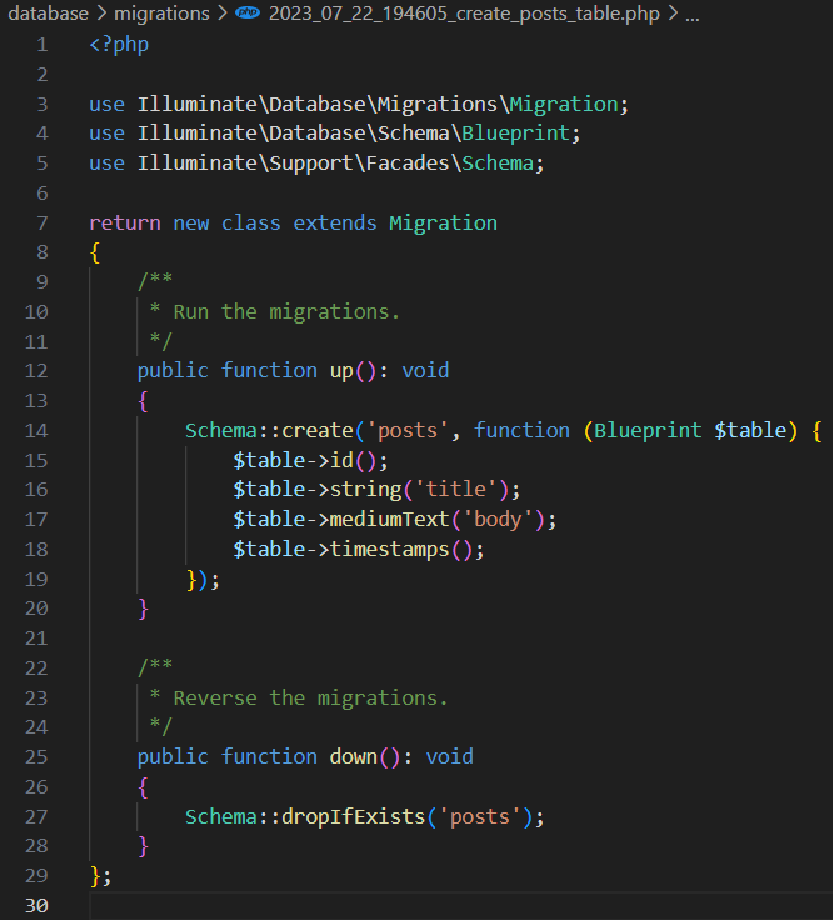
\includegraphics[width=0.5\textwidth]{figures-C1/post_migration.pdf}
    \caption{Exemple très simple de \migration{}\label{fig:basic_migration}}
\end{wrapfigure}
Quelques remarques supplémentaires:

\begin{enumerate}
    \item Par défaut, les \columns{} doivent obligatoirement posséder une valeur.
    \item On peut ajouter de nombreux paramètres aux \columns{} pour modifier leur comportements (exemple: \verb|->nullable()| pour leur permettre d'être vide).
    \item Les types des \column{} correspondent chacune à un type de valeur de \mysql{}, le ``vrai'' langage pour communiquer avec les \db{} duquel \laravel{} nous protège grâce aux \models{}, \migrations{}, \tables{} que nous venons de voir.
\end{enumerate}

Encore une fois, parcourir la doc officielle de \laravel{} permet d'en apprendre beaucoup plus que ce que tutoriel ne pourra jamais vous apprendre!

\subsubsection{Migrations: exécution}

Bon, après tant de blabla, passons à l'action. Mais avant cela, \laravel{} nous embête (pour une fois). Afin de n'avoir aucune erreur en exécutant la migration, il va falloir ajouter ces lignes dans \verb|app/Providers/AppServiceProvider.php|:

\begin{figure}[!h]
    \centering
    \begin{minipage}{0.49\textwidth}
         \centering
         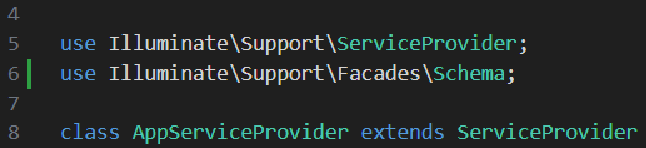
\includegraphics[width=\textwidth]{figures-C1/appservice_2.pdf}
    \end{minipage}
    \begin{minipage}{0.49\textwidth}
         \centering
         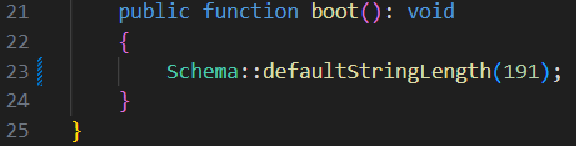
\includegraphics[width=0.95\textwidth]{figures-C1/appservice_1.pdf}
    \end{minipage}
\end{figure}

Voilà! maintenant tapez \verb|php artisan migrate:fresh --seed| (où \verb|fresh| signifie que tout ce qui existait avant est supprimé et \verb|--seed| permet d'exécuter les \texttt{seeders} vus dans la \texttt{Section~} (WIP)) et, si tout va bien, vous verrez maintenant cela en allant dans \phpmyadmin{}:

\begin{figure}[!h]
    \centering
    \begin{minipage}{0.49\textwidth}
         \centering
         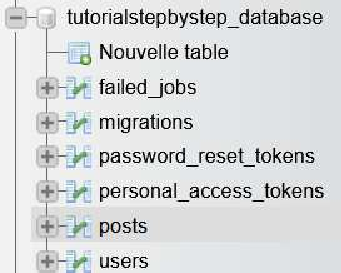
\includegraphics[width=0.6\textwidth]{figures-C1/db_posts_1.pdf}
    \end{minipage}
    \begin{minipage}{0.49\textwidth}
         \centering
         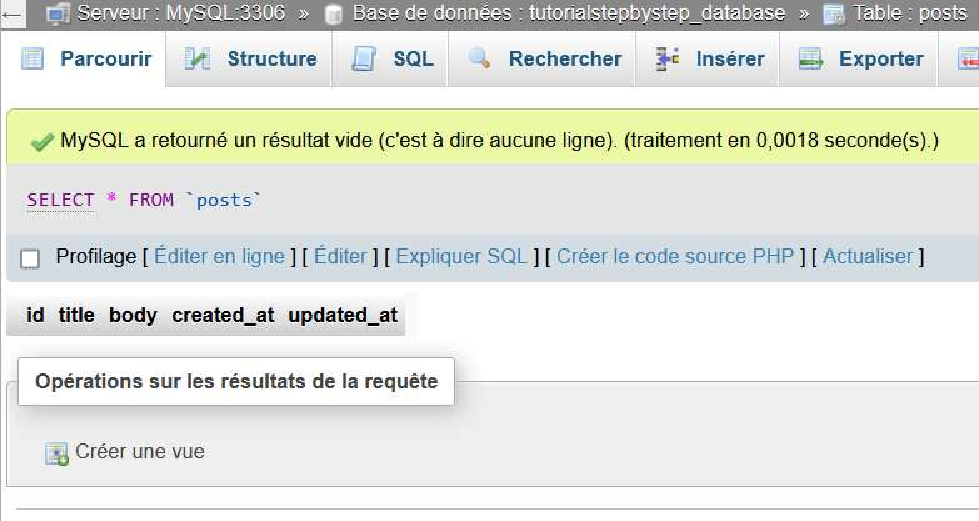
\includegraphics[width=0.9\textwidth]{figures-C1/db_posts_2.pdf}
    \end{minipage}
\end{figure}

\subsubsection[PostsController][laravel.com/docs/10.x/controllers\#resource-controllers]{PostsController}

Pour gérer ces posts, nous allons bien entendu avoir besoin d'un \controller{}. Comme ce genre de donnée va avoir des manipulations basiques très communes (création, liste, affichage, modification, suppression,\ldots), il existe un certain type de controller permettant de nous faire gagner du temps: le \texttt{resource} \controller{}. Tapez donc \\
\verb|php artisan make:controller PostsController --resource| pour en créer un.

Ensuite, il faut évidement définir des nouvelles routes. Une seule ligne toute simple nous permet de générer en réaliter 7 \routes{} différentes que nous verrons petit à petit. Ajoutez donc ces 2 lignes dans \verb|routes/web.php|:

\begin{figure}[!h]
    \centering
    \begin{minipage}{0.6\textwidth}
        \centering
        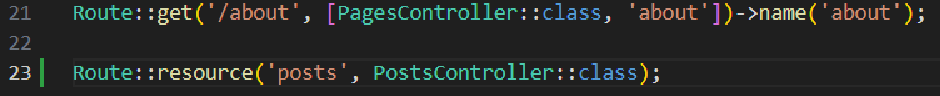
\includegraphics[width=\textwidth]{figures-C1/res_route_1.pdf}
        \caption{\label{fig:post_route}}
    \end{minipage}
    \begin{minipage}{0.38\textwidth}
        \centering
        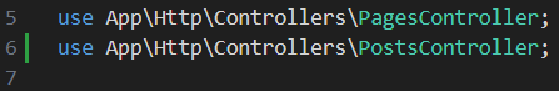
\includegraphics[width=\textwidth]{figures-C1/res_route_2.pdf}
        \caption{}
    \end{minipage}
\end{figure}
\vspace{-0.5cm}
Notez que en donnant \textit{'posts'} en argument à \verb|resource()|, celui-ci fait automatiquement lien avec le \model{} \verb|Post|\footnote{Pour comprendre comment \laravel{} fait pour être si intelligent, jetez un oeil à \href{https://laravel.com/docs/10.x/eloquent#table-names}{ceci}.}.

Petite parenthèse avant de continuer: un exemple de route générée par la commande de la \texttt{Figure~\ref{fig:post_route}} est: \\
\verb|Route::get('/posts/{post}', [PostsController::class, show])->name('posts.show')|
le \verb|{...}| dans l'URL est une sorte de paramètre dans l'URL, qui permet de passer des informations au controller. En effet, chaque paramètre dans l'URL sera passé (si on le souhaite) en argument aux fonctions du controller, dans le même ordre d'apparition que dans l'URL. Ce paramètre est extrêmement utile comme nous le verrons à la \texttt{Section~\ref{sec:post_show}}. Fin de la parenthèse.

Bon, maintenant, il faut remplir ce \controller{} et créer les \views{} qui vont avec. Commençons par les plus simples, \verb|index()| et \verb|show()|.

\subsubsubsection{index}
Cette method est utilisée pour afficher la liste de tous les Posts créés. 

\begin{wrapfigure}[5]{r}{0.4\textwidth}
    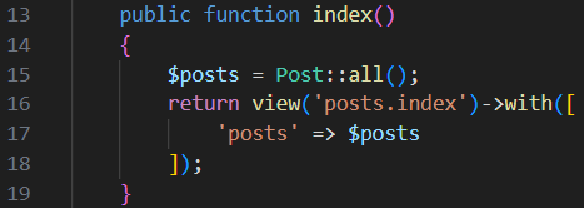
\includegraphics[width=0.4\textwidth]{figures-C1/post_index_controller.pdf}
\end{wrapfigure}
Avec cet exemple simple, on comprend vite à quel point il est simple d'intéragir avec la \db{} par l'intermédiaire des \models{}. Nos posts sont stockés sous forme d'une array d'objets \php{}, contenant les champs que nous avons spécifés dans la \migration{}. 

\SaveVerb{post_index}|index.blade.php|
\begin{wrapfigure}[11]{r}{0.581\textwidth}
    \vspace{-0.5cm}
    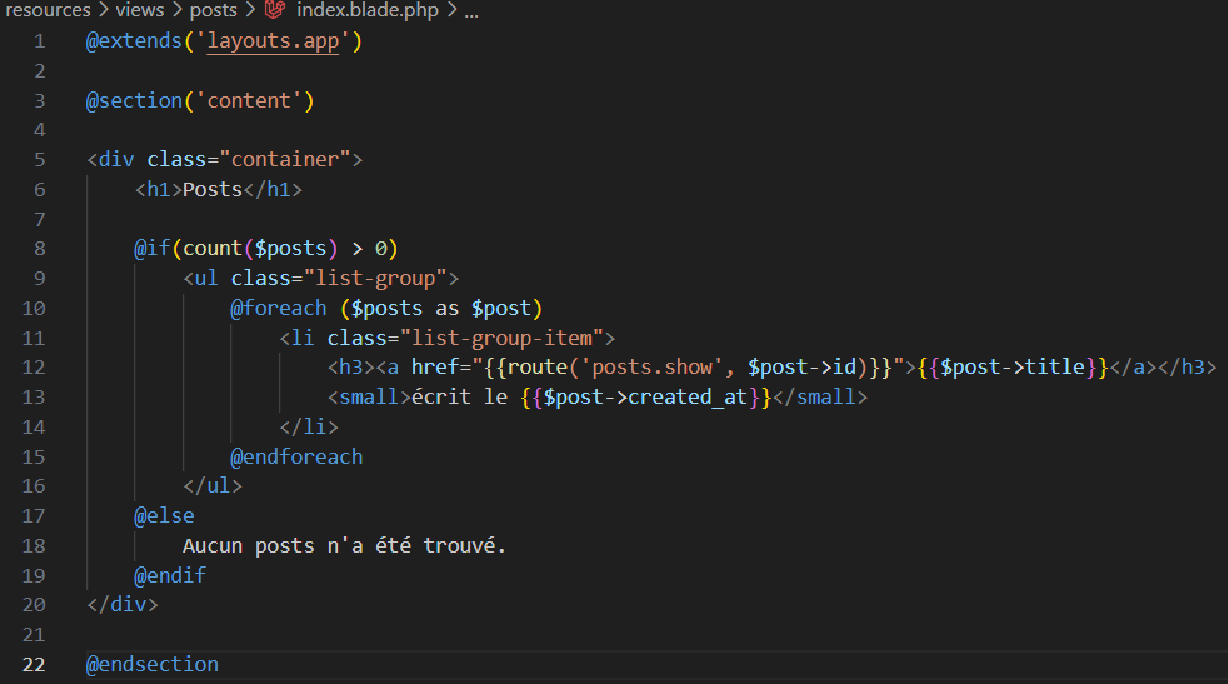
\includegraphics[width=0.581\textwidth]{figures-C1/post_index_blade.pdf}
    \caption{\protect\UseVerb{post_index}\label{fig:post_index}}
\end{wrapfigure}
Ensuite, nous allons créer un nouveau dossier \verb|posts| dans  \\ \verb|resources/views| et ajouter un fichier dedans appelé \\ \verb|index.blade.php|. Il ne reste ``plus qu'à'' le remplir avec le contenu de la \texttt{Figure~\ref{fig:post_index}}.

Ici, tout est déjà connu mis à part le \verb|@if|, mais c'est plutôt intuitif au vu de ce que je vous ai déjà appris. Ensuite, il y a le \verb|->| permettant d'accéder aux différents champs des objets que sont nos \verb|$post|.

Enfin, il ne nous reste plus qu'à ajouter un bouton à notre navbar afin d'accéder à cette page.

\begin{figure}[!h]
    \centering
    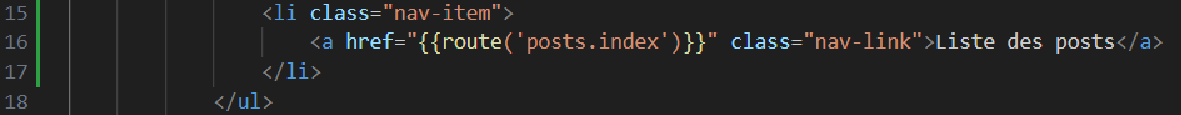
\includegraphics[width=0.75\textwidth]{figures-C1/post_index_navbar.pdf}
\end{figure}

\subsubsubsection{show}\label{sec:post_show}

Même chose que pour la page précédente, il faut remplir la fonction \verb|show()|.

\begin{wrapfigure}[5]{r}{0.4\textwidth}
    \vspace{-0.5cm}
    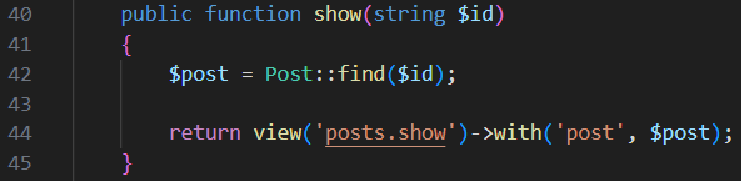
\includegraphics[width=0.4\textwidth]{figures-C1/post_show_controller.pdf}
\end{wrapfigure}
Ici, nous utilisons ce que j'ai expliqué en dessous de la \texttt{Figure~\ref{fig:post_route}}. La fonction \verb|show()| prend un argument, appelé \verb|$id|. Pourquoi et d'où sort-il? Son origine a été expliquée plus haut, il provient du paramètre \verb|{post}| dans l'URL correspondant à la fonction\footnote{Si on avait eu deux paramètres différents, par exemple \verb|.../{post}/{comment}|, et qu'on avait gardé \verb|show($id1)|, \verb|$id1| aurait pris la valeur de \verb|{post}|. Pour obtenir la valeur du deuxième paramètre on aurait du écrire \verb|show($id1, $id2)| (et \verb|$id2| aurait pris la valeur de \verb|{comment}|).}. 

Maintenant, pourquoi l'avoir appellé \verb|$id|? Simplement parce qu'il contient l'ID du post que nous souhaitons obtenir, puisque c'est la valeur que nous lui avons donné en écrivant \\ \verb|route(posts.show, $post->id$)| dans la \texttt{Figure~\ref{fig:post_index}}\footnote{Le nom du paramètre dans l'URL n'a donc aucun rapport avec le nom de la variable dans la fonction, si ce n'est que l'un donne sa valeur à l'autre}. 

\textit{\underline{PS:}} L'écriture un petit peu différente du \verb|->with()| permet de simplifier l'écriture que nous avons utilisée jusqu'ici lorsque qu'il n'y a qu'un seul élément à ajouter.

Enfin, la \blade{} corresondante peut être créée au nom et emplacement \verb|resources/views/posts/show.blade.php|:

\begin{figure}[!h]
    \centering
    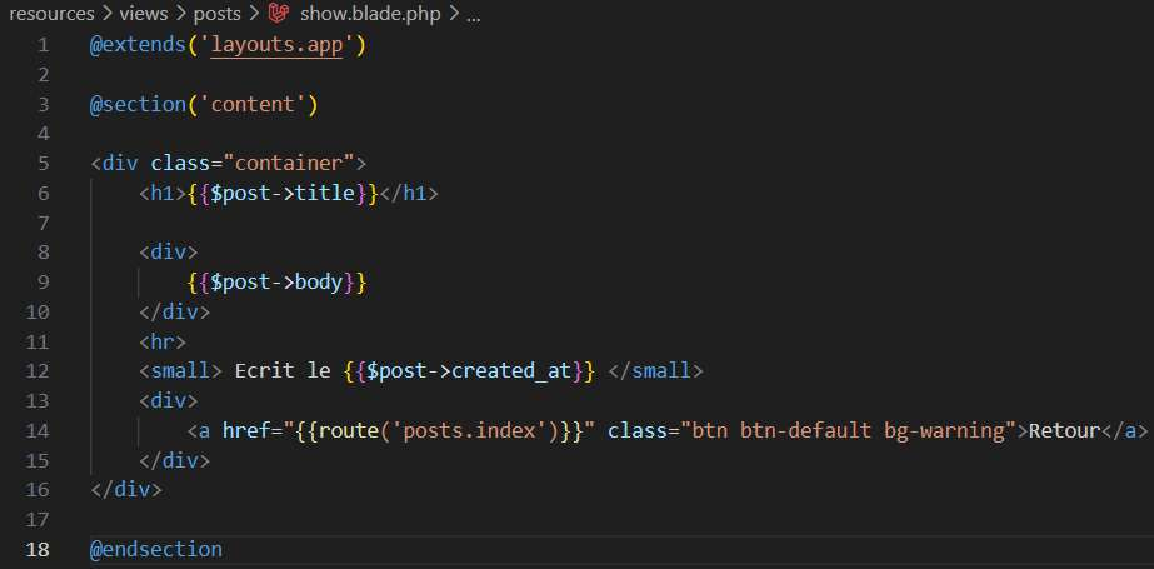
\includegraphics[width=0.75\textwidth]{figures-C1/post_show_blade.pdf}
\end{figure}

Pour le coup, R.A.S. en terme de nouveautées donc nous pouvons maintenant passer à la création de posts!

\subsubsubsection{create}

Cette partie est plus intéressante car elle va amener un nouveau concept, les \forms{}. Jusque ici, nous n'avons jamais eu à rentrer nous mêmes des données et à les envoyer à notre site pour qu'il fasse des choses avec, c'est exactement à cela que servent les \forms{}.

\begin{wrapfigure}[5]{r}{0.4\textwidth}
    \vspace{-0.5cm}
    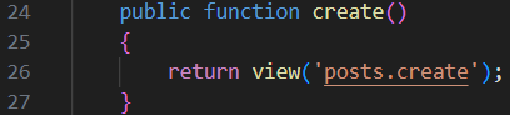
\includegraphics[width=0.4\textwidth]{figures-C1/post_create_controller.pdf}
\end{wrapfigure}
Tout d'abord, remplissons la méthode \verb|create()| du controller et créons le fichier \\ \verb|resources/posts/create.blade.php| comme nous en avons maintenant l'habitude.

Maintenant, il faut remplir la \blade:

\begin{figure}[!h]
    \centering
    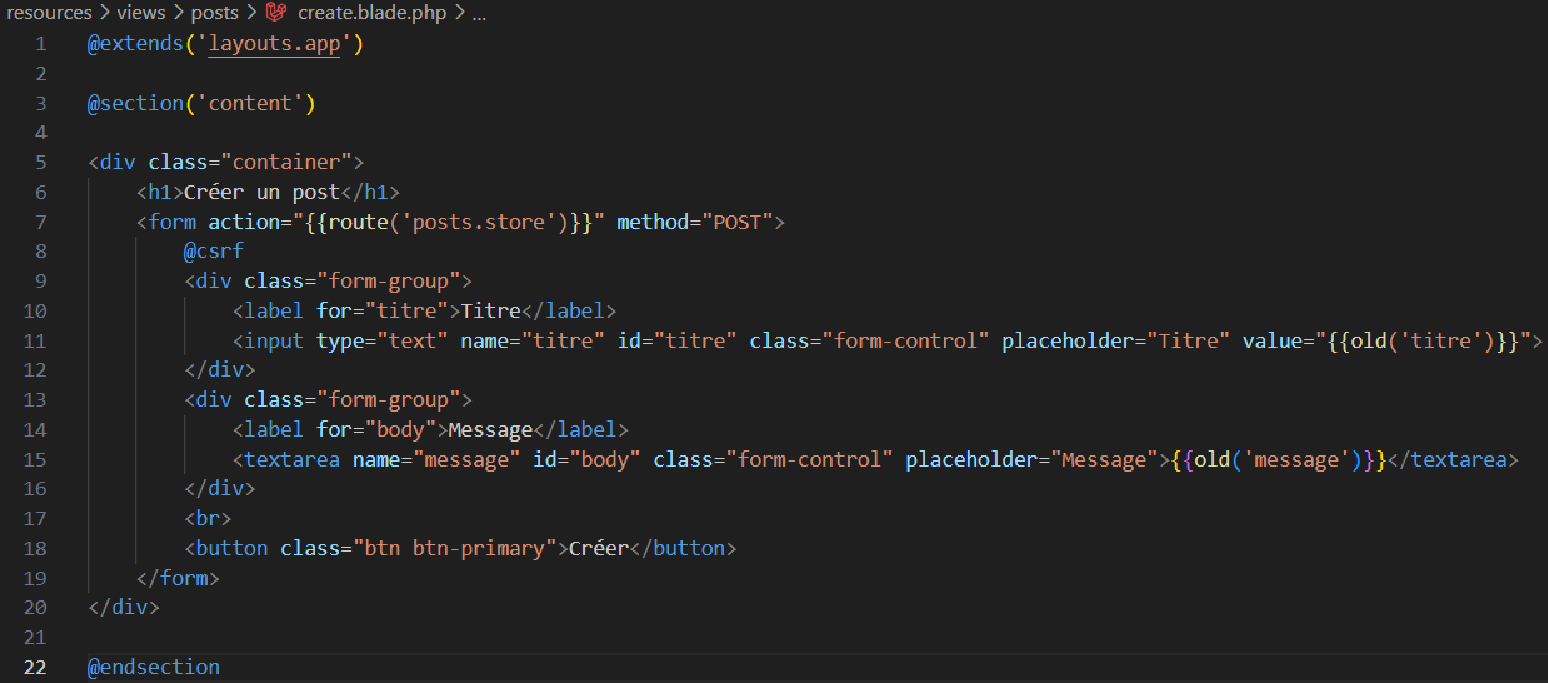
\includegraphics[width=0.8\textwidth]{figures-C1/post_create_blade.pdf}
\end{figure}
Ici il y'a pas mal de nouveautés. On voit en effet apparaitre trois nouveaux tags \html:

\begin{enumerate}
    \item \verb|<form>|: Le \form{} permet donc l'envoit d'information entrées par l'utilisateur. Pour cela, on doit lui fournir l'URL vers laquelle aller lorsque le \form{} est envoyé, c'est ce que l'on met dans \verb|action|. En l'occurence, le \texttt{resource controller} nous a créé une \route{} pour cela, appelée \verb|'posts.store'| et qui permettra de stocker les informations du \form{}. Nous verrons cela en détail à la prochaine section. Ensuite, il faut préciser le type de requête effectuée, et lorsque l'on stocke quelque chose, c'est une requête \verb|POST|\footnote{Pour afficher une \blade, on utilisait des requêtes \verb|GET|. \href{https://developer.mozilla.org/fr/docs/Web/HTTP/Methods}{Pour en savoir plus}}
    \item \verb|<label>|: Celui-ci est simplement utilisé pour donner un nom\footnote{un nom visible sur la page internet.} à un champ \verb|<input>|. Il suffit de spécifier à quel champ le \verb|<label>| fait référence en mettant le \verb|id| de l'\verb|<input>| dans l'attribut \verb|for| du \verb|<label>|.
    \item \verb|<textarea>|: Il fonctionne comme un \verb|<input>| mais est spécialisé pour la gestion de paragraphes. L'attribut \verb|value| est quant à lui substitué par l'espace entre les deux marqueurs \verb|<textarea>| et \verb|</textarea>|.
    \item \verb|<input>|: Enfin, ce tag correspond à un champ à remplir. Ce champ peut prendre plusieurs formes qui s'indiquent au moyen de l'attribut \verb|type|. En l'occurence nous utilisons un champ \verb|text| pour une petite phrase/mots (ici, le titre de notre post)\footnote{Il existe de nombreux autres types pour des fichiers, dates, boites à cocher, \ldots vous les trouverez \href{https://developer.mozilla.org/en-US/docs/Web/HTML/Element/input#input_types}{ici}.}. Les \verb|<input>| peuvent posséder de \href{https://developer.mozilla.org/en-US/docs/Web/HTML/Element/input#attributes}{très nombreux attributs}, ici nous utilisons les attributs:
    \begin{itemize}
        \item \verb|name| qui donne le nom de la variable accessible dans le \controller{}, qui contiendra les données envoyées par cet \verb|<input>|.
        \item \verb|placeholder| qui permet d'afficher un petit texte en fond dans le champ (pour par exemple donner un format de réponse)
        \item \verb|value| qui permet de donner une valeur prédéfinie au champ lorsque l'on affiche la page. Ici, \verb|old()| est une fonction prenant en argument le nom d'un \verb|<input>| et qui permet d'afficher la valeur du champ (si elle existait\footnote{on peut donner en deuxième argument à la fonction un texte à afficher lorsque le champ était vide à la requête prcédente.}) lors de la requête précédente. C'est utile lorsque les données doivent être validées avant d'être stockées (ex: est-ce que tous les champ remplis?) et que l'utilisateur est renvoyé vers la page de saisie du \form{} si la validation échoue.
    \end{itemize}
\end{enumerate}
La dernière commande inconnue est le \verb|@csrf|. C'est une mesure de sécurité contre un certain type d'attaque. Plus d'information \href{https://laravel.com/docs/10.x/csrf}{ici}.

Bon, ce fût beaucoup (trop) de bla-bla, mais on va (enfin) pouvoir passer à la suite! Promis, les trois dernières méthodes seront bien plus simples. Mais avant cela, ne pas oublier d'ajouter un bouton sur notre navbar pour accéder à cette page:

\begin{figure}[!h]
    \centering
    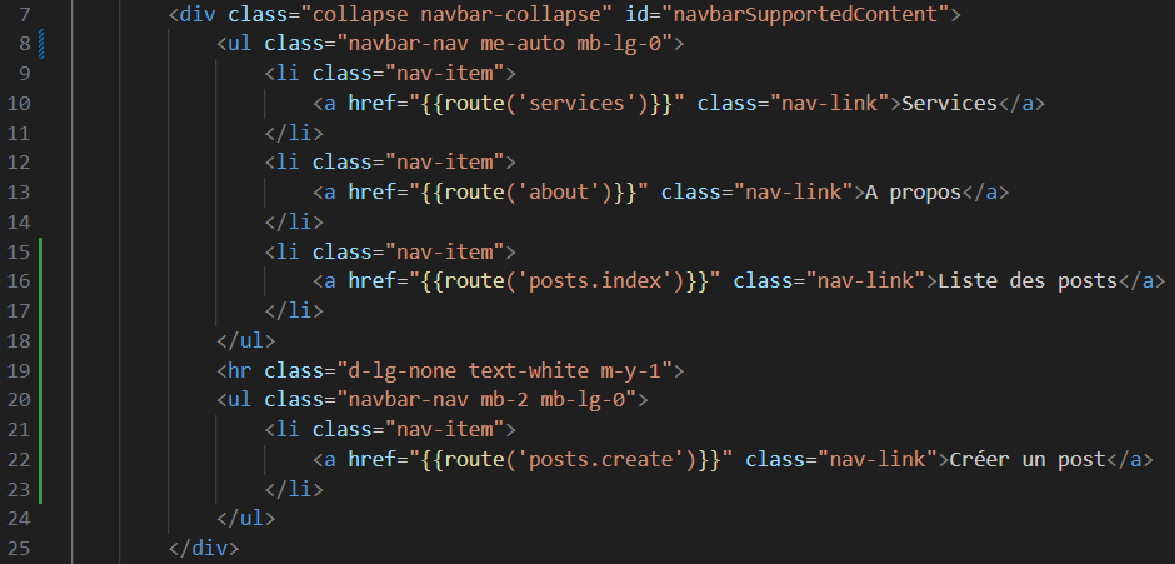
\includegraphics[width=0.75\textwidth]{figures-C1/post_create_navbar.pdf}
\end{figure}

\newpage

\subsubsubsection{store}\label{sec:posts_store}

On a vu à la section précédente que les données du \form{} étaient envoyées à la route \verb|'posts.store'|, or cette \route{} redirige vers cette fonction! C'est donc ici que nous allons stocker le post nouvellement créé.

Tout d'abord, nous allons vérifier si les 2 champs \verb|titre| et \verb|message| ont bien été remplis (s'ils doivent être remplis, ils sont requis $\Rightarrow$ \verb|required|). Pour cela, on utilise la fonction \verb|validate()| de \laravel\footnote{Plus d'informations ainsi que la liste des règles de \texttt{validation} \href{https://laravel.com/docs/10.x/validation#quick-writing-the-validation-logic}{ici}.}. Si la \texttt{validation} rate, l'utilisateur est renvoyé à la page précédente et si elle réussit, alors on continue.

\begin{wrapfigure}[9]{r}{0.7\textwidth}
    \vspace{-0.5cm}
    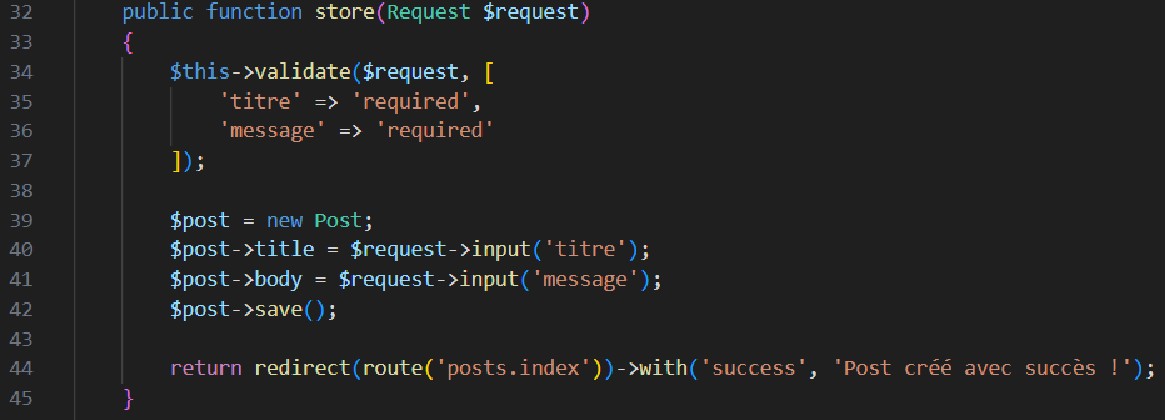
\includegraphics[width=0.7\textwidth]{figures-C1/post_store_controller.pdf}
\end{wrapfigure}
L'étape suivante est de créer un nouveau post, via son \model{}. Ensuite, on remplit ses champs avec les valeurs obtenues dans le \form{} et on le sauvegarde dans la base de donnée. Enfin, il ne reste plus qu'à envoyer l'utilisateur quelque part (la liste des posts) et le tour est joué!\footnote{La variable \verb|'success'| sera utilisée dans la \texttt{Section~\ref{sec:messages}}} Plus qu'à rajouter les fonctionnalités de modification et de suppression et puis nous en aurons terminé.

\newpage

\subsubsubsection{edit}

\begin{wrapfigure}[2]{r}{0.5\textwidth}
    \vspace{-0.5cm}
    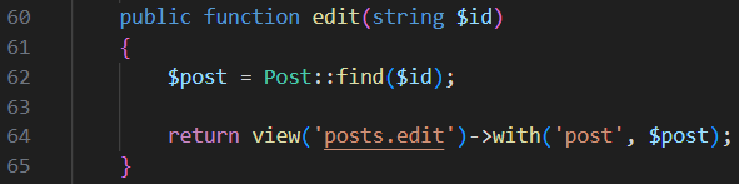
\includegraphics[width=0.5\textwidth]{figures-C1/post_edit_controller.pdf}
\end{wrapfigure}
Pour l'édition, c'est plutôt simple. Tout d'abord remplissons la méthode du \controller{}:
\vspace{1.5cm}

Ensuite, créons la \blade{} dédiée:
\begin{figure}[!h]
    \centering
    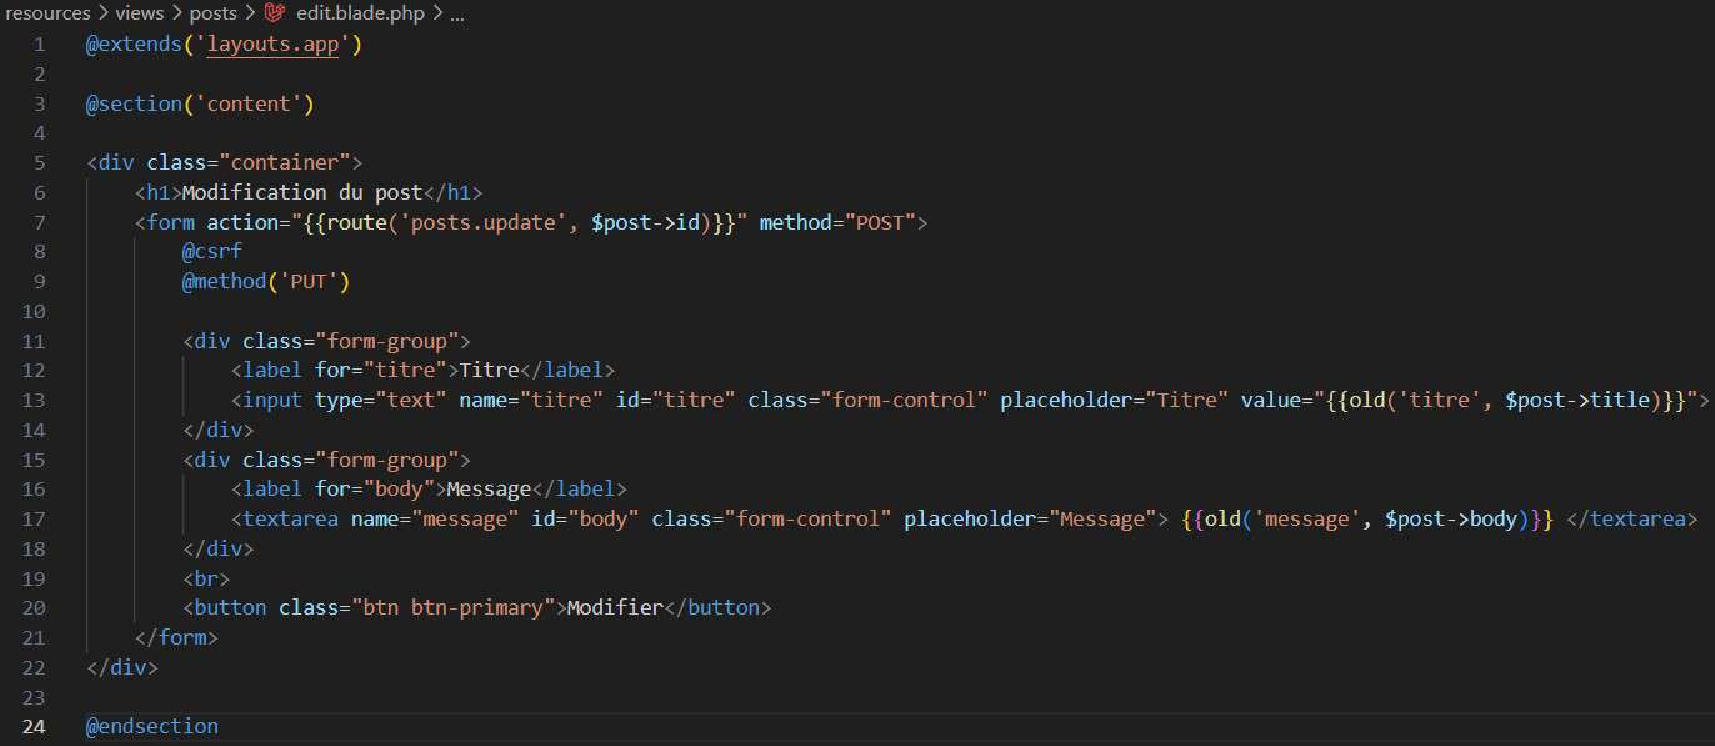
\includegraphics[width=0.75\textwidth]{figures-C1/post_edit_blade.pdf}
\end{figure}

Remarquez qu'il n'y a presque aucune différence avec la \blade{} de création de post, et c'est bien normal: on peut l'utiliser quasi à l'identique à condition de mettre les valeurs du post dans les bons champs lorsque l'on accède à la page. Une différence est néanmoins à noter, la présence du \verb|@method('PUT')|. Cette méthode permet de remplacer une donnée par une autre (notre post à modifier), mais elle n'est pas disponible directement dans les \forms{}. Il faut donc effectuer une petite accrobatie pour l'utiliser.

\subsubsubsection{update}\label{sec:posts_update}

\begin{wrapfigure}[8]{r}{0.65\textwidth}
    \vspace{-0.5cm}
    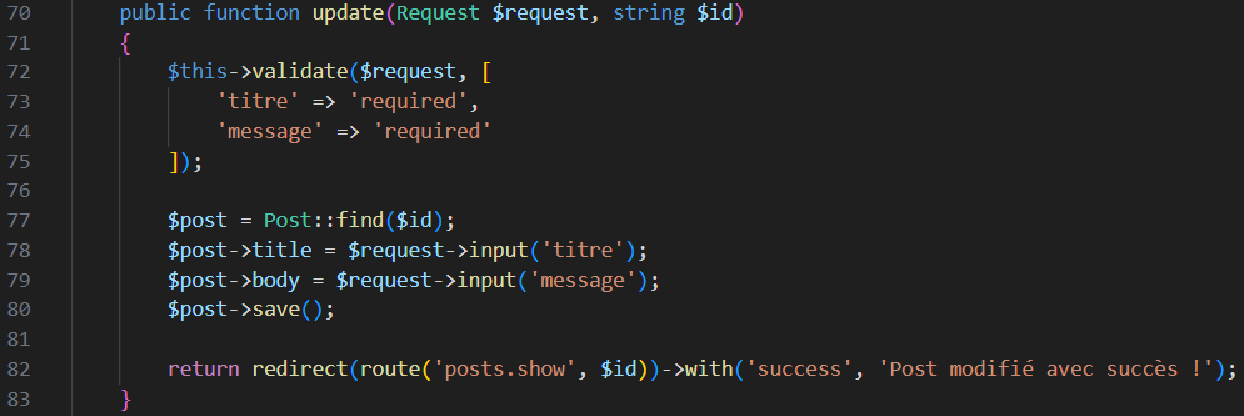
\includegraphics[width=0.65\textwidth]{figures-C1/post_update_controller.pdf}
\end{wrapfigure}
Lorsque le \form{} est envoyé, il faut bien sûr enregistrer le post dans notre \db{}. La route \verb|'posts.update'| nous envoit donc vers la méthode \verb|update()| que vous pouvez remplir comme ci-contre. Notez que ici aussi, la démarche est la même que pour la création de post (et c'est logique), mis à part qu'on cherche le post à modifier au lieu d'en créer un nouveau.

\subsubsubsection{delete}\label{sec:posts_delete}

Enfin, la suppression de post. Tout d'abord, ajoutons un bouton dans \verb|posts/show.blade.php| qui permet d'accéder à notre page de modification d'un post, un autre qui permettra de le supprimer, et stylisons un peu ces trois boutons afin qu'ils soient plaisant à voir (\texttt{Figure~\ref{fig:post_delete_blade}})

\begin{wrapfigure}[4]{r}{0.65\textwidth}
    \vspace{-0.5cm}
    \includegraphics[width=0.65\textwidth]{figures-C1/post_delete_controller.pdf}
\end{wrapfigure}
Ensuite, remplissons la méthode du \controller{}. La mécanique est ici triviale, il suffit de sélectionner le post que l'on souhaite et ensuite de le supprimer.

\begin{figure}[!h]
    \centering
    \includegraphics[width=0.75\textwidth]{figures-C1/post_delete_blade.pdf}
    \caption{\label{fig:post_delete_blade}}
\end{figure}

Et voilà! Nous avons désormais un système (simple) de création et gestion de posts! Evidément, nous pourrions rajouter énormément de fonctionnalités (commentaires, auteurs, images, \ldots). Nous explorerons certaines de ces options dans de futures sections, pour cette introduction, c'est déjà plus que suffisant.

A titre d'indication, voici le résultat auquel vous devriez arriver si tout fonctionne correctement:

\begin{figure}[!h]
    \begin{subfigure}[c]{0.73\textwidth}
        \fbox{\includegraphics[width=\textwidth]{figures-C1/posts_index.pdf}}
    \end{subfigure}\hfill
    \begin{subfigure}[c]{0.24\textwidth}
        \caption{\url{http://tutorialstepbystep/posts}} 
    \end{subfigure}
    \begin{subfigure}[c]{0.73\textwidth}
        \fbox{\includegraphics[width=\textwidth]{figures-C1/posts_show.pdf}}
    \end{subfigure}\hfill
    \begin{subfigure}[c]{0.24\textwidth}
        \caption{\url{http://tutorialstepbystep/posts/1}} 
    \end{subfigure}
    \begin{subfigure}[c]{0.73\textwidth}
        \fbox{\includegraphics[width=\textwidth]{figures-C1/posts_create.pdf}}
    \end{subfigure}\hfill
    \begin{subfigure}[c]{0.24\textwidth}
        \caption{\url{http://tutorialstepbystep/posts/create}} 
    \end{subfigure}
    \begin{subfigure}[c]{0.73\textwidth}
        \fbox{\includegraphics[width=\textwidth]{figures-C1/posts_edit.pdf}}
    \end{subfigure}\hfill
    \begin{subfigure}[c]{0.24\textwidth}
        \caption{\url{http://tutorialstepbystep/posts/1/edit}}
    \end{subfigure}
    \caption{Les quatres pages de gestions des posts.}
\end{figure}

\newpage

\subsection{Messages}\label{sec:messages}
Bon, c'est bien beau mais vous avez peut-être remarqué un gros inconvénient de notre système: lorsqu'un post est créé et qu'il manque un champ, rien ne nous dit clairement le problème! De plus, il serait profitable d'avoir une confirmation lorsqu'un post est créé/modifié/suprimé. C'est exactement à cela que vont servir les variables \verb|'success'| que nous avons créées dans la section précédente, sans les utiliser.

Créez donc un fichier \verb|resources/views/inc/messages.blade.php| et remplissez le comme sur la figure de droite.

\begin{wrapfigure}[8]{r}{0.5\textwidth}
    \vspace{-0.5cm}
    \includegraphics[width=0.5\textwidth]{figures-C1/messages_blade.pdf}
\end{wrapfigure}
Ici, les deuxième et troisième \verb|@if()| permettent de voir si la \verb|session| ($\Rightarrow$ la page actuelle, en gros) possède les variables \verb|'success'| et \verb|'error'|, et de les afficher. 

Ces variables sont celles que nous avons créées \\ aux \texttt{Section~\ref{sec:posts_store},~\ref{sec:posts_update},~\ref{sec:posts_delete}}

Enfin, le premier \verb|@if()| est utilisé afin d'afficher toutes les erreurs provenants d'un fail de validation après la soumission des \verb|<form>|.

\vspace{4cm}

Enfin, voici le résultat que vous devriez obtenir lorsque, par exemple, un post est créé (\texttt{Figure~\ref{fig:messages_create}}) ou lorsque le champ du message n'est pas rempli (\texttt{Figure~\ref{fig:messages_error}}):

\begin{figure}[!h]
    \begin{subfigure}[c]{0.42\textwidth}
        \fbox{\includegraphics[width=\textwidth]{figures-C1/messages_create.pdf}}
        \caption{\label{fig:messages_create}}
    \end{subfigure}
    \hspace{0.2cm}
    \begin{subfigure}[c]{0.52\textwidth}
        \fbox{\includegraphics[width=\textwidth]{figures-C1/messages_error.pdf}}
        \caption{\label{fig:messages_error}}
    \end{subfigure}
    \caption{}
\end{figure}








































\newpage
h
\newpage

\section{ToDo pour améliorer la formation + remarques randoms}
commande pour créer le projet avec la bonne version: \\
\verb|composer create-project laravel/laravel=^10 laravel_tutorial|
\begin{enumerate}
    \item Faire un préambule! par exemple, insister pour faire des recherches sur google
    \item faire une section avec plein de liens vers des documentations.
    \item \verb|findOrFail()| au lieu de \verb|find()| etc dans les controlers.
    \item footer avec un truc
    \item bien personnaliser les login etc
    \item envoyer des mails
    \item recaptcha
    \item changer de langue (https://laravel.com/docs/10.x/urls\#default-values) check si j'ai utilisé ca lol?
    \item CSS custom au lieu de bootstrap/ optimisation
    \item attention  prendre en compte tout ce que j'ai is dans le \verb|.txt| sur mon portable
    \item faire une listes d'extension vs code
    \item beaux messages (voir Neuro et site)
    \item error messages en dessous des inputs (voir site et neuro)
    \item améliorer la base de donnée (seeder, factories, etc)
    \item hasher toute une base de donnée (voir neuro?)
    \item softdelete? (voir neuro dans le futur)
    \item faire un easteregg avec une des URL de tutorialstepbystep?
    \item Voir photo avec \verb|active="request()->gngn"|
    \item laravel ui deprecated, => faudra passer à Breeze, soit adaptation bootstrap soit passer à Tailwind, à véfléchir.
    \item ATTENTION qd on livre un sit, pas faire \verb|npm run dev| mais \verb|npm run prod|
    \item ajouter \verb|.active| sur les \verb|.nav-link| pour indiquer la page active
\end{enumerate}

\end{document}
